\documentclass[pdflatex,sn-basic,Numbered]{sn-jnl}
\usepackage{graphicx}
\usepackage{multirow}
\usepackage{amsmath,amssymb,amsfonts}
\usepackage{booktabs,tabularx,array,url}
\usepackage[title]{appendix}
\usepackage{pgfplots,tikz}
\usetikzlibrary{shapes.geometric,arrows.meta,positioning}
\pgfplotsset{compat=1.16}
\usepackage[T1]{fontenc}
\hypersetup{hidelinks}
% generated; do not edit by hand
\newcommand{\ensAEpair}{35.77}
\newcommand{\ensAEpairLo}{33.1}
\newcommand{\ensAEpairHi}{38.2}
\newcommand{\ensAEagent}{73.20}
\newcommand{\ensAEerror}{45.79}
\newcommand{\ensHFpair}{39.72}
\newcommand{\ensHFpairLo}{37.5}
\newcommand{\ensHFpairHi}{42.1}
\newcommand{\shortAEpair}{10.75}
\newcommand{\shortAEpairLo}{9.2}
\newcommand{\shortAEpairHi}{12.4}
\newcommand{\shortHFrel}{14.30}
\newcommand{\contentAEpair}{16.79}
\newcommand{\fullAEdedup}{20.02}
\newcommand{\fullAEdedupLo}{18.5}
\newcommand{\fullAEdedupHi}{21.5}
\newcommand{\fullAErel}{26.15}
\newcommand{\fullAErelLo}{24.0}
\newcommand{\fullAErelHi}{28.4}
\newcommand{\fullHFdedup}{23.84}
\newcommand{\fullHFdedupLo}{22.3}
\newcommand{\fullHFdedupHi}{25.4}
\newcommand{\fullHFrel}{33.02}
\newcommand{\fullHFrelLo}{30.8}
\newcommand{\fullHFrelHi}{35.1}
\newcommand{\dropAE}{6.1}
\newcommand{\dropHF}{9.2}
\newcommand{\floorAE}{6.47}
\newcommand{\floorHF}{7.35}
\newcommand{\floorWW}{3.42}
\newcommand{\wwAllNo}{4.96}
\newcommand{\wwAllNoLo}{2.6}
\newcommand{\wwAllNoHi}{7.6}
\newcommand{\wwAllShift}{5.14}
\newcommand{\wwAllShiftLo}{3.2}
\newcommand{\wwAllShiftHi}{7.1}
\newcommand{\wwNameNo}{6.16}
\newcommand{\wwNameNoLo}{3.7}
\newcommand{\wwNameNoHi}{8.8}
\newcommand{\wwNameShift}{10.68}
\newcommand{\wwNameShiftLo}{8.6}
\newcommand{\wwNameShiftHi}{12.7}
\newcommand{\wwNameShiftErr}{23.12}
\newcommand{\wwAllAgent}{49.93}
\newcommand{\wwShortPair}{4.95}
\newcommand{\wwShortPairLo}{2.7}
\newcommand{\wwShortPairHi}{7.5}
\newcommand{\wwFullPair}{1.96}
\newcommand{\wwFullPairLo}{1.0}
\newcommand{\wwFullPairHi}{3.1}
\newcommand{\pubSFT}{16.62}
\newcommand{\pubSFTagent}{76.53}
\newcommand{\pubSFTerror}{27.53}
\newcommand{\pubDCL}{8.33}
\newcommand{\pubOthree}{7.86}
\newcommand{\pubOthreeWW}{7.41}
\newcommand{\pubOthreeWWagent}{53.10}
\newcommand{\pubOthreeWWerr}{14.88}
\newcommand{\dupTrain}{123}
\newcommand{\dupVal}{108}
\newcommand{\qTrain}{588}
\newcommand{\sharedConv}{451}
\newcommand{\repoQTrain}{585}
\newcommand{\repoDupTrain}{125}
\newcommand{\dupTrainPct}{20.5}
% paired label-shift gains, from aegis/results/shift_paired.json
\newcommand{\sgOldOO}{+2.68}
\newcommand{\sgOldOOLo}{+0.19}
\newcommand{\sgOldOOHi}{+5.04}
\newcommand{\sgOldOF}{+1.32}
\newcommand{\sgOldOFLo}{-0.34}
\newcommand{\sgOldOFHi}{+2.93}
\newcommand{\sgOldFO}{-1.63}
\newcommand{\sgOldFOLo}{-3.36}
\newcommand{\sgOldFOHi}{-0.12}
\newcommand{\sgOldFF}{-1.09}
\newcommand{\sgOldFFLo}{-2.51}
\newcommand{\sgOldFFHi}{+0.26}
\newcommand{\sgFullOO}{+1.64}
\newcommand{\sgFullOOLo}{-1.44}
\newcommand{\sgFullOOHi}{+4.63}
\newcommand{\sgFullOF}{+2.40}
\newcommand{\sgFullOFLo}{-0.42}
\newcommand{\sgFullOFHi}{+5.24}
\newcommand{\sgFullFO}{+0.95}
\newcommand{\sgFullFOLo}{-1.12}
\newcommand{\sgFullFOHi}{+2.95}
\newcommand{\sgFullFF}{+2.46}
\newcommand{\sgFullFFLo}{+0.39}
\newcommand{\sgFullFFHi}{+4.58}
\newcommand{\sgDdOO}{+0.19}
\newcommand{\sgDdOOLo}{-1.56}
\newcommand{\sgDdOOHi}{+1.88}
\newcommand{\sgDdOF}{+4.51}
\newcommand{\sgDdOFLo}{+1.78}
\newcommand{\sgDdOFHi}{+7.22}
\newcommand{\sgDdFO}{-0.93}
\newcommand{\sgDdFOLo}{-3.05}
\newcommand{\sgDdFOHi}{+1.16}
\newcommand{\sgDdFF}{+1.91}
\newcommand{\sgDdFFLo}{-0.16}
\newcommand{\sgDdFFHi}{+3.92}
\newcommand{\sdOldOO}{-2.49}
\newcommand{\sdOldOOLo}{-4.65}
\newcommand{\sdOldOOHi}{-0.22}
\newcommand{\sdOldOF}{+3.20}
\newcommand{\sdOldOFLo}{+0.59}
\newcommand{\sdOldOFHi}{+5.92}
\newcommand{\sdFullOO}{-1.45}
\newcommand{\sdFullOOLo}{-4.70}
\newcommand{\sdFullOOHi}{+1.77}
\newcommand{\sdFullOF}{+2.12}
\newcommand{\sdFullOFLo}{-0.71}
\newcommand{\sdFullOFHi}{+5.01}
% robustness numbers, from robustness_stats.json, name_audit.json, ensemble_size.json
\newcommand{\nmDyMis}{109}
\newcommand{\nmDyTot}{200}
\newcommand{\nmMacMis}{6}
\newcommand{\nmAgentExact}{73.20}
\newcommand{\nmAgentNorm}{80.05}
\newcommand{\nmAgentNormLo}{78.1}
\newcommand{\nmAgentNormHi}{81.9}
\newcommand{\nmPairNorm}{38.90}
\newcommand{\nmPairNormLo}{36.6}
\newcommand{\nmPairNormHi}{41.2}
\newcommand{\nmDyAgentExact}{35.6}
\newcommand{\nmDyAgentNorm}{76.2}
\newcommand{\nmDistinctIds}{429}
\newcommand{\sdAEpair}{0.20}
\newcommand{\sdWWallPair}{1.12}
\newcommand{\sdWWnameShiftPair}{2.18}
\newcommand{\ptAEallNeither}{+3.93}
\newcommand{\ptAEallNeitherLo}{+2.54}
\newcommand{\ptAEallNeitherHi}{+5.34}
\newcommand{\ptAEallNames}{+3.00}
\newcommand{\ptWWnameShiftP}{$<$0.001}
\newcommand{\ptWWnameShiftVsAll}{+5.72}
\newcommand{\ptWWnameShiftVsAllLo}{+2.74}
\newcommand{\ptWWnameShiftVsAllHi}{+8.58}
\newcommand{\sensAEmin}{33.40}
\newcommand{\sensAEhalf}{28.33}
\newcommand{\sensShiftMin}{10.26}
\newcommand{\sensShiftMax}{10.69}
\newcommand{\ensSingleAE}{31.66}
\newcommand{\ensSingleAEsd}{0.45}
\newcommand{\ensKtwoAE}{33.79}
\newcommand{\ensKfourAE}{35.07}
\newcommand{\ensKsevenAE}{35.34}
\newcommand{\ensKfourteenAE}{35.77}
\newcommand{\ensSingleWWshift}{9.73}
\newcommand{\ensSingleWWshiftSd}{1.35}
\newcommand{\ensFourteenWWshift}{10.68}
\newcommand{\costFeat}{3.1}
\newcommand{\costHead}{35.9}
\newcommand{\costInf}{0.39}
\newcommand{\costParams}{476{,}431}
% reproduction check, from baselines_dedup.json
\newcommand{\rpQwPair}{8.01}
\newcommand{\rpQwAgent}{49.24}
\newcommand{\rpQwError}{20.15}
\newcommand{\rpQwWWpair}{2.98}
\newcommand{\rpQwWWagent}{35.16}
\newcommand{\rpQwWWerror}{6.23}
\newcommand{\pubQwPair}{5.02}
\newcommand{\pubQwAgent}{27.55}
\newcommand{\pubQwError}{14.96}
\newcommand{\pubDCLagent}{22.93}
\newcommand{\pubDCLerror}{24.73}
\newcommand{\pubDCLwwAgent}{8.40}
\newcommand{\pubDCLwwError}{14.67}
\newcommand{\pubDCLwwPair}{1.60}
\newcommand{\rpDclPair}{12.64}
\newcommand{\rpDclAgent}{63.64}
\newcommand{\rpDclError}{30.88}
\newcommand{\rpDclPairLo}{11.6}
\newcommand{\rpDclPairHi}{13.7}
\newcommand{\rpDclWWpair}{3.01}
\newcommand{\rpDclWWagent}{38.12}
\newcommand{\rpDclWWerror}{11.02}
\newcommand{\floorAEagent}{62.00}
\newcommand{\floorHFagent}{68.58}
% query-cluster bootstrap, from cluster_bootstrap.json
\newcommand{\clAEgroups}{422}
\newcommand{\clAEpairLo}{33.2}
\newcommand{\clAEpairHi}{38.3}
\newcolumntype{Y}{>{\raggedright\arraybackslash}X}
\raggedbottom
% sn-jnl wraps every table in threeparttable, which breaks boxing a tabular; use the plain float (no table footnotes are used here)
\renewenvironment{table}[1][]{\begin{tableorg}[#1]\centering}{\end{tableorg}}
\newsavebox{\fitbox}
\newcommand{\fitfinish}{\ifdim\wd\fitbox>\textwidth\resizebox{\textwidth}{!}{\usebox{\fitbox}}\else\usebox{\fitbox}\fi}

\begin{document}

\title[Failure attribution in LLM-based multi-agent systems]{Failure attribution in LLM-based multi-agent systems: an audit of AEGIS-Bench and transfer to natural failures}

\author*[1]{\fnm{Aryan} \sur{Mahajan}}\email{aryan.mahajan.ug23@nsut.ac.in}
\author[1]{\fnm{Yogesh} \sur{Kumar}}\email{yogesh.kumar.ug23@nsut.ac.in}
\author[1]{\fnm{Shubham} \sur{Yadav}}\email{shubham.yadav.ug23@nsut.ac.in}
\author[1]{\fnm{Savita} \sur{Yadav}}\email{savita.yadav@nsut.ac.in}

\affil*[1]{\orgdiv{Department of Computer Science and Engineering}, \orgname{Netaji Subhas University of Technology}, \orgaddress{\city{New Delhi}, \country{India}}}
\abstract{When a multi-agent system built from large language models (LLMs) fails, which agent is to blame, and what went wrong? AEGIS-Bench offers 9,533 injected failures for training and testing, and Who\&When offers 184 natural ones. We ask how far AEGIS-Bench scores can be trusted, using the benchmark authors' published results as the reference. First, \dupTrain{} of the 600 Hugging Face test conversations (\dupTrainPct\%) are verbatim copies of training records; removing them from training costs one fixed model \dropAE{} pair micro-F1 points on the authors' test file and \dropHF{} on the Hugging Face file. Second, a model that never reads the conversation, and sees only agent name, framework and turn counts, reaches \shortAEpair{} pair micro-F1 (95\% interval \shortAEpairLo--\shortAEpairHi) on the authors' file, above the authors' own contrastive method (\pubDCL) and every published zero-shot LLM row. Third, a fine-tuned ensemble of 14 encoders trained on duplicate-free data reaches \ensAEpair{} pair and \ensAEerror{} error micro-F1, above the authors' fine-tuned 14B model (\pubSFT{} and \pubSFTerror), but behind it at the agent level (\ensAEagent{} against \pubSFTagent). Fourth, on Who\&When the same ensemble scores \wwAllNo{} pair micro-F1 with all feature blocks, no better than the model that ignores the text; label-shift correction helped clearly only under a block mask we chose after seeing Who\&When (\wwNameNo{} to \wwNameShift). Fifth, \nmDyMis{} of \nmDyTot{} gold agent labels in one framework differ from the speaker names only in letter case, which exact matching cannot credit. A scorer test against the authors' code supports the comparison.}

\keywords{multi-agent systems, large language models, failure attribution, benchmark leakage, shortcut learning, label shift}

\maketitle

\section{Introduction}
Multi-agent systems built on large language models (MAS) hand pieces of a task to cooperating agents, and people have used them for reasoning, software engineering and scientific work~\cite{wu,hong,du,qian}. That division of labour makes them fragile. One agent's mistake can travel through the following turns, so the failure we finally see may sit far from where it began. To understand a failed run, then, we need to say which agents were responsible and what kind of mistake each one made. Cemri et al.\ sorted the recurring failures of MAS into 14 modes in three groups~\cite{mast}, and Zhang et al.\ posed automated failure attribution on natural failure logs~\cite{whowhen}.

Natural failures are hard to collect, since an expert has to read and label every log. The version of Who\&When we use has only 184 annotated records~\cite{whowhen}. Much recent work has turned to injected failures instead: take a successful run, replay it with a deliberate error, and the label is known for free. AEGIS~\cite{aegis} built 9,533 such trajectories with agent and failure-mode labels, and AgenTracer~\cite{agentracer}, CORRECT-Error~\cite{correct} and Who\&When Pro~\cite{whenpro} take similar routes. That fixes the shortage of data but raises a new question. Models trained on injected failures are meant for natural ones, and several recent audits suspect that injected benchmarks contain artefacts and shortcuts~\cite{audit1,audit2,catch}.

We audit one of these benchmarks, AEGIS-Bench, and look at how well a small trained attributor carries over from it to natural failures. We hold ourselves to one rule: the only outside numbers we compare with are the ones the benchmark's authors published, quoted as they reported them, and every claim of our own comes with a control that a reader can check. Our five research questions are these.
\begin{itemize}
\item \textbf{RQ1.} How much of an AEGIS-Bench score survives duplicate removal, and what do a trivial floor and a no-text baseline say about published rows?
\item \textbf{RQ2.} Under the deduplicated protocol (published training data minus test duplicates), how does a stronger fine-tuned ensemble compare with the published rows?
\item \textbf{RQ3.} How large is the gap between in-domain and natural (Who\&When) attribution, and does hiding feature blocks (block-dropout) narrow it?
\item \textbf{RQ4.} Does correcting for a shifted failure-mode mix (label shift) help, and when does it fail?
\item \textbf{RQ5.} Do framework-adversarial training and a cheap frozen LLM judge help (earlier study, as logged)?
\end{itemize}
Our contributions are as follows.
\begin{enumerate}
\item \textbf{Duplicate leakage and an agent-name inconsistency} in the released AEGIS files, with their effect on scores (Section~\ref{sec:leak}).
\item \textbf{A shortcut-only baseline, trivial floors and record-level intervals} that place the published rows in context (Section~\ref{sec:shortcut}).
\item \textbf{A like-for-like comparison} with published rows: the published training data minus test duplicates, and a scorer shown to match the authors' (Section~\ref{sec:main}).
\item \textbf{A negative and a conditional transfer result} on Who\&When: all-blocks transfer is at the shortcut-only level, and label shift helps clearly under one post hoc mask only, with an effect that differs across training configurations (Section~\ref{sec:ww}).
\item \textbf{Controlled negative results} for adversarial framework removal and a frozen judge, reported as logged with their limits (Section~\ref{sec:legacy}).
\end{enumerate}
The closest prior audit of AEGIS-Bench, by Xu and Gao~\cite{audit2}, scores zero-shot judges against speaker-name-only predictors at the agent level and notes a name-format issue in its test conversations. We did not find a duplicate audit of the released AEGIS files, a pair-level no-text baseline compared with published rows, or EM label-shift correction applied to failure attribution, but our literature search was limited (Section~\ref{sec:limits}).

\section{Related Work}
Table~\ref{tab:related} lists the closest prior work and what each piece leaves open for our questions.

\subsection{Multi-agent LLM systems and their failures}
Representative MAS include conversational frameworks~\cite{wu}, role-based software teams~\cite{hong}, multi-agent debate~\cite{du}, networked topologies~\cite{qian}, dynamic agent networks~\cite{dylan}, hierarchical role assignment~\cite{agentverse}, orchestrator--executor systems~\cite{magentic} and tool-using agents~\cite{smol}. MAST analyses over 1,600 annotated traces from seven frameworks and derives the 14-mode taxonomy that AEGIS reuses, finding that many failures come from system design and coordination~\cite{mast}. TRAIL annotates agentic traces with located issues~\cite{trail}.

\subsection{Failure attribution on natural and injected data}
Who\&When~\cite{whowhen} was the first to ask for the responsible agent and the decisive step, using logs from 127 MAS; its authors report low step-level accuracy. AEGIS~\cite{aegis} brings a large injected dataset, supervised and reinforcement fine-tuning of LLMs, and DCL, a small contrastive model. AgenTracer~\cite{agentracer} trains a tracer on counterfactually replayed and fault-injected trajectories. CORRECT~\cite{correct} needs no training and instead retrieves schemata distilled from past failures. AFANet~\cite{afanet}, still a preprint, uses a light graph network and mentions test-time adaptation. Who\&When Pro~\cite{whenpro} simply adds more injected data.

\subsection{Validity of injected benchmarks and shortcut learning}
Models often succeed on a benchmark by using cues that correlate with the label~\cite{geirhos}. For failure attribution, three recent audits are close to ours. Xu and Gao~\cite{audit2} test whether judge scores reflect cues: on three benchmarks, simple predictors match or beat GPT-4.1, and on AEGIS-Bench a predictor that blames every speaker matches GPT-4.1 on agent-level micro-F1 (49.2 against 50.0) but trails on exact-set accuracy. They evaluate 600 AEGIS conversations from one Hugging Face revision (107 of which no longer appear in the current release), report that 275 of 417 annotated names that match no speaker differ only by case or whitespace, use zero-shot GPT-4.1 as the only judge and run no trained model on AEGIS. Pal et al.~\cite{audit1} audit whether an injected-failure benchmark picks the same monitor as natural failures, on synthetic enterprise audit bundles rather than AEGIS-Bench. CatchBench~\cite{catch} shows that a rule reading only declaration order can reach perfect F1 on one configuration source, which supports checking labels for shortcuts. We read the first paper in full through a summarising tool, the second in its main text, and the third at abstract level. We add a duplicate and overlap audit of the released AEGIS files, trained models compared with published rows, a pair-level no-text baseline with file-specific floors, and transfer of a trained model to natural failures.

\subsection{Label shift, calibration and adaptation}
Label (prior) shift, in which the class mix changes while the class-conditional input distribution does not, can be corrected with an EM procedure~\cite{saerens} or with bias-corrected calibration~\cite{alexandari}; both depend on calibrated predictions~\cite{guo}. Domain-adversarial training removes domain information from features by gradient reversal~\cite{ganin}. Feature-block dropout is a variant of dropout~\cite{dropout} and modality dropout~\cite{moddrop}.

\subsection{LLM judges and research gaps}
LLM-as-a-judge scores outputs with a prompted model and depends on option position and prompt format~\cite{zheng}. We see four gaps. Each is worded as ``we did not find'', since our search was limited and some sources are preprints. \textbf{G1:} a duplicate audit of the released AEGIS files, and a pair-level no-text baseline compared with published rows (agent-level speaker-name predictors exist~\cite{audit2}). \textbf{G2:} a like-for-like comparison with the published AEGIS rows that removes test duplicates from training. \textbf{G3:} the failure-mode mix treated as a label shift for attribution. \textbf{G4:} a map of which input blocks a small attributor relies on and what happens when they are hidden.

\begin{table*}[t]
\caption{Closest related work and the dimensions covered by this study.}
\label{tab:related}
\centering\footnotesize
\begin{tabularx}{\textwidth}{@{}l Y Y Y@{}}
\toprule
Work & Contribution & Evaluated on & Gap relative to this study \\
\midrule
MAST~\cite{mast} & 14-mode failure taxonomy, annotated traces & 1,600+ traces, 7 frameworks & Taxonomy only; no trained attributor \\
Who\&When~\cite{whowhen} & Natural failures with responsible agent and step; prompting methods & 127 MAS; 184 records in the version used & Small; low step accuracy \\
TRAIL~\cite{trail} & Trace issue localisation & Annotated agentic traces & Small; no injected-to-natural transfer \\
AEGIS~\cite{aegis} & Injected dataset; SFT, RL, DCL & 9,533 injected trajectories; Who\&When out of domain & Released files overlap; test file not named; no shortcut baseline \\
AgenTracer~\cite{agentracer} & Counterfactual replay and fault injection; RL-trained tracer & Own data; Who\&When & Step level; LLM-sized model \\
CORRECT~\cite{correct} & Training-free error schemata retrieved at inference & Injected set; Who\&When & Judge-style; no shift analysis \\
AFANet~\cite{afanet} (preprint) & Lightweight GNN; test-time adaptation & AEGIS-Bench; Who\&When & Single remedy; no duplicate or shortcut controls \\
Who\&When Pro~\cite{whenpro} & Larger injected benchmark & Injected failures & More injected data; no transfer study \\
Audits~\cite{audit1,audit2,catch} & Validity and shortcut checks; speaker-name-only predictors on AEGIS~\cite{audit2} & Judges; AEGIS agent level only~\cite{audit2}; other benchmarks & No duplicate audit, trained model, pair-level no-text baseline or published-row comparison \\
\textbf{This work} & Duplicate audit, floors, no-text baseline, deduplicated-protocol ensemble, block masks, label shift & AEGIS-Bench (two test files); Who\&When & --- \\
\bottomrule
\end{tabularx}
\end{table*}

\section{Task, Data and Protocol}\label{sec:protocol}
\subsection{Task and metrics}
A multi-agent trajectory $\tau$ ends in a failure. Its label is a set of (agent, failure-mode) pairs over the 14 MAST modes~\cite{mast,aegis}. A model predicts a set of such pairs. Following~\cite{aegis}, we report micro-F1 at three levels. At the pair level a prediction is correct only if both agent and mode match; at the agent level only the faulty agents are scored, and at the error level only the modes. With $P_i$ and $G_i$ the predicted and gold sets of record $i$ at a given level,
\begin{equation}
\mathrm{F1}_{\text{micro}}=\frac{2\sum_i |P_i\cap G_i|}{\sum_i |P_i|+\sum_i |G_i|}.
\end{equation}
Micro-F1 pools counts over all records, so frequent labels dominate. All scores are percentages.

\subsection{Datasets}
AEGIS-Bench~\cite{aegis} contains 9,533 injected trajectories from six frameworks (AgentVerse, DyLAN, Debate, MacNet, Magentic-One, SmolAgents) over six task families; an LLM manipulator injects errors into otherwise successful runs, so labels are known by construction. Who\&When~\cite{whowhen} provides 184 natural failure records, each with exactly one faulty agent, free-form agent names, and free-text mistake reasons that we map to the 14 modes with the preprocessing of~\cite{aegis}. This yields a skewed mode mix, with FM-2.6 at about 26\% and FM-3.3 at about 21\% of labels. Twenty labels name an agent that never speaks in the logged turns, so the maximum agent recall is about 89\%. Table~\ref{tab:data} lists the roles.

\begin{table}[t]
\caption{Datasets and their role.}
\label{tab:data}
\centering\footnotesize
\begin{tabularx}{\columnwidth}{@{}Y l Y@{}}
\toprule
Dataset & Records & Role \\
\midrule
AEGIS-Bench, released split & 7,146 / 1,787 / 600 & Train, validation, test (Hugging Face file) \\
AEGIS-Bench, authors' file & 600 (100 per benchmark) & Test \\
Deduplicated protocol & 6,912 / 1,657 & Train, validation \\
Who\&When & 184 & Out-of-domain test only \\
\bottomrule
\end{tabularx}
\end{table}

\subsection{Dataset statistics}
In the released training split (7,146 records) the most frequent mode (FM-1.1) has 1,632 labelled instances and the least frequent (FM-3.1) 1,004, so the injected mode mix is close to balanced. In the 3,865-record query-disjoint subset used by the earlier study the counts are 954 for FM-1.1 and 529 for FM-2.6, the least frequent mode there. Who\&When averages about 3.7 agents per record, and about 27\% of agents are faulty. FM-2.6 and FM-3.3 account for about 47\% of its labels, and FM-2.6 is the most frequent mode there (about 26\%). This gap between a near-uniform injected mix and a skewed natural mix motivates the label-shift correction. Because each Who\&When record has exactly one faulty agent, a single wrong record changes pair micro-F1 by about half a point, which is why the intervals in Table~\ref{tab:ww} are wide.

\subsection{Two test files}
The authors' repository contains \texttt{aegis.jsonl} with 100 records per benchmark (GSM8K, HumanEval, MATH, MMLU, SciBench and GAIA split 40 + 60), which matches the description in~\cite{aegis}. The Hugging Face \texttt{test.jsonl} has 600 records but a different benchmark mix (105, 105, 105, 105 and 104 records for five benchmarks, 76 for GAIA). The two files share no record ids but \sharedConv{} identical conversations. A concurrent audit reports that 107 of 600 conversations in an earlier Hugging Face revision of the test file are absent from the current release~\cite{audit2}, so the Hugging Face file itself has changed over time. The published paper does not name its test file, so we report both, with the authors' file primary because it matches the description.

\subsection{Scope and design choices}\label{sec:scope}
Four choices limit what we can claim. First, we use one injected and one natural benchmark. AEGIS-Bench is the largest injected set with both agent and mode labels, and Who\&When is the natural set AEGIS itself tests on out of domain, so our transfer results can be read against published rows. Second, we use one encoder family. MiniLM is small enough to fine-tune 14 times on free GPUs and to retrain heads on a CPU, which is what made ensembles, block masks and intervals affordable; we say nothing about larger encoders. Third, published rows are our reference, because our question is whether published numbers mean what they seem to mean. Every comparison therefore uses the benchmark authors' scorer and published rows, and only our own models are run under their protocol. Re-running their fine-tuned 14B models would add variation from prompts, decoding and parsing, and we could not afford it. We did run two lighter published baselines, a zero-shot Qwen2.5-7B and a DCL-style encoder, as a reproduction check (Section~\ref{sec:repro}). Fourth, AgenTracer, CORRECT and AFANet report different tasks, metrics or data, so we cite them but keep their numbers out of our tables. The baselines in Tables~\ref{tab:aegis} and~\ref{tab:aegishf} thus come from a single source, which Section~\ref{sec:limits} counts as a limitation.

\subsection{Scorer parity}
We re-implemented the metric and checked it against the authors' \texttt{evaluate.py}. On 200 random datasets, and on a full JSONL run through the authors' \texttt{evaluate\_results}, micro and macro F1 agree to $10^{-12}$. A third test pins down the one place where the two differ: the authors skip non-list predictions, while our harness counts them as empty. We also broke the scorer on purpose to confirm that this test fails when it should.

\subsection{Deduplicated protocol: released training data minus test duplicates}
We train on the released training split and tune on the released validation split, but drop every record whose conversation also occurs in either test file. Conversation identity is the SHA-1 of agent name and content over all turns. This leaves 6,912 training and 1,657 validation records, from 7,146 and 1,787. This is conservative, since the published models were presumably trained with the duplicates. We call this the \emph{deduplicated protocol}, and the unmodified released data the \emph{released protocol}.

\subsection{Out-of-domain protocol}
Who\&When labels are never used for training, tuning, thresholds or retrieval. Thresholds and early stopping use only AEGIS validation. The data loader never reads annotation fields such as the number of injected agents, ground-truth fields or per-turn injection flags. Because Who\&When has 184 records, one record is worth about 0.5 pair points, and we report record-level bootstrap intervals (2,000 resamples, 95\%) throughout and treat differences inside the intervals as noise.

\subsection{Floors and baselines}
The \emph{trivial floor} predicts every agent present with all 14 modes. It needs no model, and any score near it carries no evidence of skill. It scores \floorAE{} on the authors' file, \floorHF{} on the Hugging Face file and \floorWW{} on Who\&When (pair micro-F1). The \emph{frequency baseline} predicts each agent's most common modes. The \emph{shortcut-only} baseline sees only agent name, framework and turn counts, and the \emph{content-only} baseline sees only the conversation text vectors.

\section{Methods}\label{sec:methods}
\subsection{Per-agent features and head}
Each (trajectory, agent) row concatenates five blocks. The content block is the mean turn vector of that agent, from all-MiniLM-L6-v2~\cite{minilm,sbert} at 256 tokens. The name block is an embedding of the agent name, which gives a handle on roles such as ``solver'' or ``critic'' without a fixed vocabulary. The framework block is a one-hot of the six frameworks. The peer block holds the agent mean minus the mean of the other agents' turns, the agent mean minus the query vector and four cosine similarities, so it measures how an agent deviates from its peers. The count block has turn-count scalars. A two-hidden-layer MLP (256 units each) predicts a faulty-agent probability $p_a$ and 14 mode probabilities $p_{a,m}$.

\subsection{Models}
The \emph{frozen} model is this head on frozen embeddings (5 seeds). The \emph{fine-tuned ensemble} uses 14 independently fine-tuned MiniLM encoders (seeds 0--13), each trained end to end with binary cross-entropy on the 14 mode outputs and a faulty-agent output (settings in Table~\ref{tab:settings}). Early stopping uses a 15\% hold-out of the training data (1,068 records), so the validation split stays untouched and 5,844 records remain for gradient updates. Validation loss was lowest at epoch 3 or 4 in all runs (best loss 0.130 to 0.134), and one epoch took about 222 s on a free Kaggle T4 GPU. All 101,009 turn texts are then re-embedded with each fine-tuned encoder, and three MLP heads per encoder are trained on the saved vectors on a CPU.

\subsection{Block-dropout}
Agent names, framework identity and peer statistics help in-domain, but Who\&When agent names are free-form and its structure differs. We train each head on four copies of the training data: both blocks on, name block zeroed, peer block zeroed, and both zeroed. At test time any mask can be applied. Probabilities are averaged over encoders for each head seed and mask, thresholds are tuned on AEGIS validation with the same mask, and one model therefore serves all four masks. This extends name-dropout in the spirit of~\cite{dropout,moddrop}.

\subsection{Decoder and ensembling}
A pair $(a,m)$ is output when $p_a\ge t_a$ and $p_{a,m}\ge t_m$, with both global thresholds tuned on validation. If nothing fires, the top pair of the record is returned. For Who\&When we keep the standard decoder; the one-faulty-agent structure of the benchmark is not used in the headline rows.

\subsection{Label-shift correction}
Let $\pi_s$ be the training mode prior. For a record $r$ define a raw mode distribution $q_r(m)\propto\sum_a p_a p_{a,m}$ from the model's own predictions. Following Saerens et al.~\cite{saerens}, we estimate the target prior $\hat\pi$ by EM on the unlabelled target records. Starting from $\hat\pi=\pi_s$ we iterate
\begin{equation}
q'_r(m)=\frac{\hat\pi_m/\pi_{s,m}\,q_r(m)}{\sum_{m'}\hat\pi_{m'}/\pi_{s,m'}\,q_r(m')},\quad \hat\pi_m\leftarrow\frac1{|R|}\sum_r q'_r(m)
\end{equation}
until $\hat\pi$ stops changing. The final weights $\hat\pi_m/\pi_{s,m}$ are normalised to mean one, clipped so that probabilities stay at most 1, and multiply each mode probability before decoding with the unchanged AEGIS-tuned thresholds. The method assumes calibrated predictions~\cite{alexandari,guo} and an unchanged $P(\text{text}\mid\text{mode})$. It is \emph{transductive}: it reads the unlabelled Who\&When inputs, though never their labels.

\subsection{Earlier-study components}
The earlier study (Section~\ref{sec:legacy}) also used framework-adversarial training and a frozen LLM judge. The adversary is a classifier that predicts the six frameworks from the pooled agent vector through a gradient-reversal layer~\cite{ganin}, with weights $\lambda=0.5$ and $1.0$, with and without name-dropout. For the judge, the trained ensemble proposes the top-$k$ pairs per record ($k=5$ in study 1, $k=12$ in study 2), and a frozen 4-bit Qwen2.5-7B-Instruct~\cite{qwen} answers ``did agent A commit mode M?'' for each candidate. The score is the log-odds of the two answer tokens, averaged over swapped option order to reduce position bias~\cite{zheng}. The fused score is the model logit plus $w$ times the judge score, with $w\in\{0,0.25,0.5,1,2\}$ chosen by 2-fold cross-fitting on AEGIS validation. Gates, success criteria and the scoring script were committed before any test or Who\&When score was computed.

\begin{figure}[t]
\centering
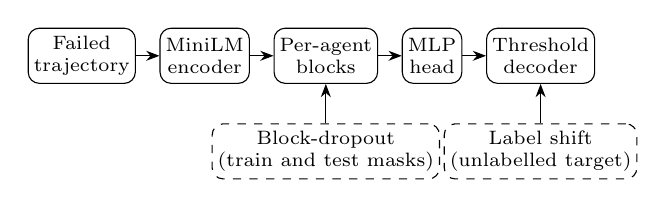
\begin{tikzpicture}[node distance=3mm,box/.style={draw,rounded corners,align=center,font=\scriptsize,minimum height=7mm,inner sep=2pt}]
\node[box] (a) {Failed\\trajectory};
\node[box,right=of a] (b) {MiniLM\\encoder};
\node[box,right=of b] (c) {Per-agent\\blocks};
\node[box,right=of c] (d) {MLP\\head};
\node[box,right=of d] (e) {Threshold\\decoder};
\draw[-{Stealth}] (a)--(b);\draw[-{Stealth}] (b)--(c);\draw[-{Stealth}] (c)--(d);\draw[-{Stealth}] (d)--(e);
\node[box,below=5mm of c,dashed] (f) {Block-dropout\\(train and test masks)};
\node[box,below=5mm of e,dashed] (g) {Label shift\\(unlabelled target)};
\draw[-{Stealth}] (f)--(c);\draw[-{Stealth}] (g)--(e);
\end{tikzpicture}
\caption{Pipeline. Per-agent blocks (content, name, framework, peer, counts) feed an MLP head and a threshold decoder tuned on AEGIS validation. Block masks act on the blocks; label shift reweights mode probabilities before decoding}
\label{fig:pipe}
\end{figure}

\section{Duplicate Leakage}\label{sec:leak}
In the released files, \qTrain{} of the 600 Hugging Face test records share a query with a training record, and \dupTrain{} (\dupTrainPct\%) test conversations are word-for-word copies of training conversations (\dupVal{} for validation). The authors' file overlaps the released training data too: \repoQTrain{} of its 600 records share a query with a training record, and \repoDupTrain{} conversations are verbatim. AEGIS makes several faulty variants of each task, so a model can pick up what a task is about instead of where the fault is. The AEGIS paper describes its subsets as non-overlapping~\cite{aegis}. We only claim that the \emph{released files} overlap.

Table~\ref{tab:leak} shows the effect on one fixed frozen model: removing the duplicates from training lowers pair micro-F1 by \dropAE{} points on the authors' file and \dropHF{} on the Hugging Face file, with non-overlapping intervals. The effect is a property of the files; whether the published rows were trained with the duplicates is not stated.

\subsection{Agent-name mismatch in the authors' file}\label{sec:names}
A second property of the authors' file affects scores directly. Scoring is by exact string match on agent names, and in this file \nmDyMis{} of the \nmDyTot{} gold agent labels of DyLAN records are lowercase (\texttt{assistant1}) while the speakers in the same conversation are \texttt{Assistant1}. \nmMacMis{} MacNet labels differ from the speaker by a hyphen (\texttt{Node2} against \texttt{Node-2}). All of these match a speaker once case, hyphens and underscores are ignored. We found no such mismatch in the 16,586 training labels or in the Hugging Face file, so a model trained on the released data names agents as they speak and can never be credited for these labels. The file also has only \nmDistinctIds{} distinct record ids among its 600 records, so ids cannot serve as keys. Xu and Gao~\cite{audit2} also report case and whitespace mismatches (275 of 417 mismatching occurrences in their 600 conversations); we add the per-framework count, the absence of mismatches elsewhere, and the effect on a trained model. Table~\ref{tab:names} shows that agent micro-F1 on the authors' file is \nmAgentExact{} under exact matching and \nmAgentNorm{} (\nmAgentNormLo--\nmAgentNormHi) under normalised matching, and on DyLAN alone \nmDyAgentExact{} against \nmDyAgentNorm. Pair micro-F1 rises from \ensAEpair{} to \nmPairNorm{} (\nmPairNormLo--\nmPairNormHi). We keep exact matching for every headline number, because it is the published scorer's rule and we do not know how the published generative models named agents; the normalised figures are a sensitivity analysis. The DyLAN weakness reported in Section~\ref{sec:main} is therefore mostly a label-format effect, and any comparison of agent-level scores on this file, including ours with Aegis-SFT, depends on how labels are matched.

\begin{table}[t]
\caption{Agent names in the authors' test file. Gold agent labels that equal no speaker name in their own conversation, by framework (none in the 16,586 training labels or the Hugging Face file), and the ensemble's micro-F1 (\%) under exact and normalised (case, hyphen and underscore ignored) name matching. Mean over three head seeds.}
\label{tab:names}
\centering\footnotesize\setlength{\tabcolsep}{2pt}
\begin{lrbox}{\fitbox}\begin{tabular}{@{}lrrrr@{}}
\toprule
 & Unmatched & Agent ex. & Agent norm. & Pair norm. \\
\midrule
DyLAN (87 rec.) & 109 of 200 & 35.6 & 76.2 & 39.7 \\
MacNet (100 rec.) & 6 of 393 & 75.8 & 76.6 & 37.2 \\
All 600 rec. & 115 of 1320 & 73.2 & 80.0 & 38.9 \\
\bottomrule
\end{tabular}\end{lrbox}\fitfinish
\end{table}

% generated; do not edit by hand
\begin{table*}[t]
\caption{AEGIS-Bench, authors' test file (primary). Micro-F1 (\%); ``rep.'' = copied from Table~1 of~\cite{aegis}; ``ours'' = run by us with 95\% record-level bootstrap intervals. Our training data have the test duplicates removed (Section~\ref{sec:protocol}).}
\label{tab:aegis}
\centering\footnotesize\setlength{\tabcolsep}{3pt}
\begin{lrbox}{\fitbox}\begin{tabular}{@{}llrrr@{}}
\toprule
Model & Src. & Pair & Agent & Error \\
\midrule
Random & rep. & 0.33 & 4.54 & 11.23 \\
Qwen2.5-7B (zero-shot) & rep. & 5.02 & 27.55 & 14.96 \\
GPT-4.1 (zero-shot) & rep. & 7.44 & 37.48 & 20.65 \\
o3 (zero-shot) & rep. & 7.86 & 40.31 & 22.37 \\
DCL & rep. & 8.33 & 22.93 & 24.73 \\
Aegis-SFT & rep. & 16.62 & 76.53 & 27.53 \\
Aegis-GRPO & rep. & 6.84 & 49.74 & 21.19 \\
\midrule
Trivial floor & ours & 6.47 {\scriptsize[6.2, 6.7]} & 62.00 {\scriptsize[59.7, 64.3]} & 26.19 {\scriptsize[25.4, 27.0]} \\
Frequency baseline & ours & 10.77 {\scriptsize[10.0, 11.5]} & 69.55 {\scriptsize[66.7, 72.2]} & 27.24 {\scriptsize[26.3, 28.2]} \\
Shortcut-only (no text) & ours & 10.75 {\scriptsize[9.2, 12.4]} & 58.35 {\scriptsize[55.5, 61.2]} & 23.54 {\scriptsize[21.5, 25.7]} \\
Content-only & ours & 16.79 {\scriptsize[15.5, 18.0]} & 69.62 {\scriptsize[66.9, 72.3]} & 30.89 {\scriptsize[29.3, 32.4]} \\
Full, frozen encoder, 1 model & ours & 20.02 {\scriptsize[18.5, 21.5]} & 68.45 {\scriptsize[65.6, 71.0]} & 31.43 {\scriptsize[29.7, 33.0]} \\
\textbf{Fine-tuned, 14 encoders} & ours & 35.77 {\scriptsize[33.1, 38.2]} & 73.20 {\scriptsize[70.2, 76.0]} & 45.79 {\scriptsize[43.3, 48.0]} \\
\bottomrule
\end{tabular}\end{lrbox}\fitfinish
\end{table*}

\begin{table*}[t]
\caption{AEGIS-Bench, Hugging Face test file (secondary), same models as Table~\ref{tab:aegis}. Micro-F1 (\%) with 95\% intervals.}
\label{tab:aegishf}
\centering\footnotesize\setlength{\tabcolsep}{3pt}
\begin{lrbox}{\fitbox}\begin{tabular}{@{}lrrr@{}}
\toprule
Model & Pair & Agent & Error \\
\midrule
Trivial floor & 7.35 {\scriptsize[7.1, 7.6]} & 68.58 {\scriptsize[67.1, 70.0]} & 27.14 {\scriptsize[26.4, 27.9]} \\
Frequency baseline & 12.81 {\scriptsize[12.0, 13.5]} & 80.45 {\scriptsize[79.2, 81.7]} & 28.87 {\scriptsize[27.9, 29.9]} \\
Shortcut-only (no text) & 11.74 {\scriptsize[10.3, 13.3]} & 68.37 {\scriptsize[66.6, 70.1]} & 24.93 {\scriptsize[22.9, 26.9]} \\
Content-only & 18.77 {\scriptsize[17.6, 19.9]} & 75.17 {\scriptsize[73.7, 76.6]} & 32.60 {\scriptsize[31.1, 34.0]} \\
Full, frozen encoder, 1 model & 23.84 {\scriptsize[22.3, 25.4]} & 79.13 {\scriptsize[77.6, 80.5]} & 34.13 {\scriptsize[32.4, 35.8]} \\
\textbf{Fine-tuned, 14 encoders} & 39.72 {\scriptsize[37.5, 42.1]} & 84.31 {\scriptsize[82.8, 85.9]} & 47.58 {\scriptsize[45.4, 49.8]} \\
\bottomrule
\end{tabular}\end{lrbox}\fitfinish
\end{table*}

\begin{table}[t]
\caption{Effect of verbatim duplicates on one model (frozen MiniLM, flat MLP, 5 seeds). Pair micro-F1 (\%) with 95\% intervals. ``Released'' trains on the released train/validation data; ``deduplicated'' removes every record whose conversation also occurs in a test file.}
\label{tab:leak}
\centering\footnotesize\setlength{\tabcolsep}{3pt}
\begin{lrbox}{\fitbox}\begin{tabular}{@{}lrrr@{}}
\toprule
Test file & Released & Deduplicated & Drop \\
\midrule
Authors' file & 26.15 {\scriptsize[24.0, 28.4]} & 20.02 {\scriptsize[18.5, 21.5]} & 6.13 \\
Hugging Face file & 33.02 {\scriptsize[30.8, 35.1]} & 23.84 {\scriptsize[22.3, 25.4]} & 9.19 \\
\bottomrule
\end{tabular}\end{lrbox}\fitfinish
\end{table}

\begin{table*}[t]
\caption{What the score is made of (frozen MiniLM, flat MLP, 5 seeds, deduplicated training data). Pair micro-F1 (\%) with 95\% intervals; shortcut-only sees agent name, framework and turn counts but never the text.}
\label{tab:shortcut}
\centering\footnotesize\setlength{\tabcolsep}{3pt}
\begin{lrbox}{\fitbox}\begin{tabular}{@{}lrrr@{}}
\toprule
Input & Authors' file & HF file & Who\&When \\
\midrule
Trivial floor & 6.47 {\scriptsize[6.2, 6.7]} & 7.35 {\scriptsize[7.1, 7.6]} & 3.42 {\scriptsize[3.1, 3.8]} \\
Shortcut-only & 10.75 {\scriptsize[9.2, 12.4]} & 11.74 {\scriptsize[10.3, 13.3]} & 4.95 {\scriptsize[2.7, 7.5]} \\
Content-only & 16.79 {\scriptsize[15.5, 18.0]} & 18.77 {\scriptsize[17.6, 19.9]} & 2.71 {\scriptsize[1.6, 3.9]} \\
Full & 20.02 {\scriptsize[18.5, 21.5]} & 23.84 {\scriptsize[22.3, 25.4]} & 1.96 {\scriptsize[1.0, 3.1]} \\
\bottomrule
\end{tabular}\end{lrbox}\fitfinish
\end{table*}

\begin{table*}[t]
\caption{Who\&When (184 natural failures, out-of-domain; no Who\&When label is used for training or tuning). Micro-F1 (\%); intervals are 95\% record-level bootstrap. Label shift reads unlabelled Who\&When inputs (transductive). $^\dagger$ mask chosen after seeing Who\&When results (post hoc).}
\label{tab:ww}
\centering\footnotesize\setlength{\tabcolsep}{3pt}
\begin{lrbox}{\fitbox}\begin{tabular}{@{}llrrr@{}}
\toprule
Model & Src. & Pair & Agent & Error \\
\midrule
Random & rep. & 0.11 & 1.06 & 8.74 \\
DCL & rep. & 1.60 & 8.40 & 14.67 \\
Aegis-SFT & rep. & 4.03 & 51.14 & 9.87 \\
GPT-4.1 (zero-shot) & rep. & 3.36 & 42.29 & 7.00 \\
o3 (zero-shot) & rep. & 7.41 & 53.10 & 14.88 \\
\midrule
Trivial floor & ours & 3.42 {\scriptsize[3.1, 3.8]} & 38.32 {\scriptsize[35.0, 41.8]} & 13.33 {\scriptsize[13.3, 13.3]} \\
Shortcut-only (1 model) & ours & 4.95 {\scriptsize[2.7, 7.5]} & 38.08 {\scriptsize[33.2, 43.0]} & 10.87 {\scriptsize[7.5, 14.7]} \\
Full, frozen encoder (1 model) & ours & 1.96 {\scriptsize[1.0, 3.1]} & 33.88 {\scriptsize[29.0, 39.2]} & 7.63 {\scriptsize[5.6, 10.0]} \\
14 encoders, all blocks & ours & 4.96 {\scriptsize[2.6, 7.6]} & 49.93 {\scriptsize[44.8, 55.3]} & 7.96 {\scriptsize[4.8, 11.3]} \\
\quad + label shift & ours & 5.14 {\scriptsize[3.2, 7.1]} & 51.69 {\scriptsize[47.8, 55.7]} & 10.28 {\scriptsize[7.5, 13.1]} \\
14 encoders, peer block hidden$^\dagger$ & ours & 6.16 {\scriptsize[3.7, 8.8]} & 51.03 {\scriptsize[46.7, 55.3]} & 12.56 {\scriptsize[9.2, 16.0]} \\
\quad + label shift$^\dagger$ & ours & 10.68 {\scriptsize[8.6, 12.7]} & 51.27 {\scriptsize[47.8, 54.8]} & 23.12 {\scriptsize[19.5, 26.6]} \\
\bottomrule
\end{tabular}\end{lrbox}\fitfinish
\end{table*}
\begin{table*}[t]
\caption{Test-time block masks, 14-encoder ensemble (3 head seeds): pair micro-F1 (\%) with 95\% record-level bootstrap intervals. Label shift is applied to Who\&When only.}
\label{tab:gridci}
\centering\footnotesize\setlength{\tabcolsep}{3pt}
\begin{lrbox}{\fitbox}\begin{tabular}{@{}lcccc@{}}
\toprule
Name / peer block & Authors' file & HF file & Who\&When & + shift \\
\midrule
on / on & 35.77 {\scriptsize[33.1, 38.2]} & 39.72 {\scriptsize[37.5, 42.1]} & 4.96 {\scriptsize[2.6, 7.6]} & 5.14 {\scriptsize[3.2, 7.1]} \\
on / off$^\dagger$ & 32.77 {\scriptsize[30.4, 35.1]} & 36.61 {\scriptsize[34.5, 38.8]} & 6.16 {\scriptsize[3.7, 8.8]} & 10.68 {\scriptsize[8.6, 12.7]} \\
off / on & 34.93 {\scriptsize[32.4, 37.4]} & 38.37 {\scriptsize[36.1, 40.7]} & 4.71 {\scriptsize[2.3, 7.5]} & 3.78 {\scriptsize[2.0, 5.8]} \\
off / off & 31.84 {\scriptsize[29.4, 34.3]} & 34.88 {\scriptsize[32.7, 37.1]} & 4.77 {\scriptsize[2.6, 7.4]} & 6.67 {\scriptsize[4.8, 8.7]} \\
\bottomrule
\end{tabular}\end{lrbox}\fitfinish
\end{table*}

\section{What the Score Is Made Of}\label{sec:shortcut}
Table~\ref{tab:shortcut} separates inputs. A model that sees only agent name, framework and turn counts reaches \shortAEpair{} pair micro-F1 (\shortAEpairLo--\shortAEpairHi) on the authors' file, against a floor of \floorAE{} and a content-only model at \contentAEpair. Under the released protocol the shortcut-only model reaches \shortHFrel{} on the Hugging Face file. These exceed published DCL (\pubDCL) and every published zero-shot LLM row (at most \pubOthree). One caveat: our model is trained on AEGIS and the published LLMs are zero-shot. What we claim is that the benchmark's shortcuts are strong enough to beat weak published rows, not that those methods are bad. Xu and Gao~\cite{audit2} report a related agent-level result with speaker-name-only predictors (49.2 micro-F1 against 50.0 for zero-shot GPT-4.1); ours differs in scoring pairs, in using framework and turn counts, in being trained, and in being compared with published rows on named files. The floor depends on the file (\floorAE{} on the authors' file, \floorHF{} on the Hugging Face file, \floorWW{} on Who\&When), so a score must be read against the floor of its own file.

\section{Comparison with Published Rows}\label{sec:main}
Tables~\ref{tab:aegis} and~\ref{tab:aegishf} and Fig.~\ref{fig:aegis} compare the 14-encoder ensemble with published rows copied from Table~1 of~\cite{aegis}. On the authors' file the ensemble reaches \ensAEpair{} pair micro-F1 (\ensAEpairLo--\ensAEpairHi) and \ensAEerror{} error micro-F1, against \pubSFT{} and \pubSFTerror{} for Aegis-SFT, a 14B model. It does \emph{not} win at the agent level under exact matching (\ensAEagent{} against \pubSFTagent); with normalised names (Section~\ref{sec:names}) it scores \nmAgentNorm{}, but the published rows were produced under exact matching, so we keep the exact figure. A frozen single model scores \fullAEdedup{} (\fullAEdedupLo--\fullAEdedupHi) on the same file, so most of the gain over it comes from fine-tuning and ensembling. The comparison is like-for-like in training data under the deduplicated protocol but not in test-file knowledge, since the published paper does not name its file, and the published models are larger and generative while ours are small encoders with agent-name features. All this shows is that a small model with these features holds its own in-domain; it does not show an architectural advantage.

\begin{table*}[t]
\caption{All 25 published rows copied as reported from Table~1 of~\cite{aegis}: micro / macro F1 (\%) at pair, agent and error level, on AEGIS-Bench (AB) and Who\&When (WW). Not recomputed by us.}
\label{tab:pubfull}
\centering\tiny\setlength{\tabcolsep}{2.5pt}
\begin{lrbox}{\fitbox}\begin{tabular}{@{}lrrrrrrrrrrrr@{}}
\toprule
 & \multicolumn{6}{c}{AEGIS-Bench} & \multicolumn{6}{c}{Who\&When} \\
\cmidrule(lr){2-7}\cmidrule(lr){8-13}
Model & Pair mi & Pair ma & Agent mi & Agent ma & Err mi & Err ma & Pair mi & Pair ma & Agent mi & Agent ma & Err mi & Err ma \\
\midrule
Random & 0.33 & 0.21 & 4.54 & 3.56 & 11.23 & 11.15 & 0.11 & 0.05 & 1.06 & 0.83 & 8.74 & 7.14 \\
DCL (Ours) & 8.33 & 5.30 & 22.93 & 20.23 & 24.73 & 27.70 & 1.60 & 0.77 & 8.40 & 6.07 & 14.67 & 10.57 \\
only-mix head & 5.17 & 4.20 & 24.33 & 22.60 & 25.20 & 26.80 & 1.20 & 0.60 & 9.40 & 6.07 & 12.77 & 10.67 \\
only-bilinear & 2.67 & 2.40 & 14.60 & 14.00 & 24.33 & 24.17 & 0.60 & 0.53 & 7.03 & 5.43 & 12.97 & 11.40 \\
w/o intent & 5.43 & 6.83 & 13.70 & 13.90 & 22.67 & 23.80 & 1.10 & 0.55 & 8.00 & 5.90 & 11.00 & 9.00 \\
w/o consistency & 2.93 & 2.80 & 14.47 & 13.67 & 23.47 & 23.20 & 0.50 & 0.43 & 6.27 & 5.20 & 11.80 & 9.50 \\
Qwen2.5-7B-Instruct & 5.02 & 2.52 & 27.55 & 14.49 & 14.96 & 11.36 & 2.31 & 1.14 & 40.92 & 23.50 & 3.64 & 1.77 \\
Qwen2.5-7B-Instruct {+} SFT & 5.05 & 2.80 & 60.03 & 22.70 & 19.61 & 16.90 & 1.26 & 0.52 & 43.51 & 32.51 & 6.77 & 4.20 \\
Qwen2.5-7B-Instruct {+} GRPO & 7.11 & 2.77 & 35.43 & 14.86 & 17.21 & 10.54 & 2.31 & 1.19 & 50.77 & 30.14 & 3.86 & 2.30 \\
Qwen2.5-14B-Instruct & 5.47 & 2.20 & 35.78 & 12.71 & 20.24 & 5.91 & 0.00 & 0.00 & 49.88 & 33.19 & 1.56 & 1.35 \\
Qwen2.5-14B-Instruct {+} SFT (Aegis-SFT) & 16.62 & 9.99 & 76.53 & 47.97 & 27.53 & 27.66 & 4.03 & 2.08 & 51.14 & 36.94 & 9.87 & 7.77 \\
Qwen2.5-14B-Instruct {+} GRPO (Aegis-GRPO) & 6.84 & 2.55 & 49.74 & 18.38 & 21.19 & 16.10 & 2.45 & 1.49 & 54.43 & 40.88 & 4.15 & 2.67 \\
Qwen3-8B-Non-Thinking & 3.96 & 1.40 & 21.34 & 8.16 & 15.81 & 13.89 & 3.88 & 1.81 & 27.78 & 17.64 & 3.88 & 1.91 \\
Qwen3-8B-Non-Thinking {+} SFT & 9.68 & 5.73 & 64.79 & 38.96 & 20.37 & 20.36 & 5.17 & 2.33 & 45.48 & 30.77 & 8.00 & 5.29 \\
Qwen3-8B-Non-Thinking {+} GRPO & 6.94 & 2.82 & 45.91 & 17.39 & 20.89 & 15.15 & 2.21 & 1.45 & 50.94 & 38.26 & 2.21 & 1.68 \\
Qwen3-8B-Thinking & 4.42 & 1.52 & 34.63 & 9.01 & 17.48 & 14.31 & 1.95 & 1.10 & 37.91 & 27.58 & 4.65 & 2.21 \\
Qwen3-8B-Thinking {+} GRPO & 4.41 & 1.66 & 36.11 & 15.73 & 17.94 & 12.03 & 8.10 & 3.19 & 53.12 & 40.52 & 11.25 & 6.91 \\
Qwen2.5-72B-Instruct & 5.60 & 2.20 & 37.46 & 14.51 & 17.72 & 16.58 & 3.56 & 2.11 & 44.44 & 26.05 & 5.59 & 4.34 \\
gpt-oss-120b & 6.53 & 1.71 & 38.58 & 5.53 & 20.38 & 12.05 & 8.09 & 3.30 & 51.56 & 35.41 & 14.75 & 6.98 \\
GPT-4.1 & 7.44 & 2.27 & 37.48 & 11.12 & 20.65 & 15.75 & 3.36 & 1.16 & 42.29 & 28.93 & 7.00 & 5.84 \\
GPT-4o-mini & 5.76 & 1.63 & 38.54 & 14.72 & 19.95 & 16.02 & 2.11 & 0.98 & 47.42 & 34.21 & 5.26 & 3.33 \\
o3 & 7.86 & 2.27 & 40.31 & 23.27 & 22.37 & 16.76 & 7.41 & 3.98 & 53.10 & 42.55 & 14.88 & 8.63 \\
Gemini-2.5-Flash & 6.99 & 2.76 & 42.02 & 16.45 & 23.47 & 19.85 & 7.32 & 3.33 & 55.56 & 36.98 & 11.94 & 7.96 \\
Gemini-2.5-Pro & 6.96 & 2.88 & 41.32 & 16.15 & 19.93 & 16.29 & 6.81 & 2.69 & 53.11 & 34.92 & 11.07 & 8.11 \\
Claude-Sonnet-4 & 7.68 & 2.34 & 40.73 & 15.51 & 21.21 & 16.55 & 6.77 & 2.66 & 44.76 & 37.23 & 13.33 & 9.23 \\
\bottomrule
\end{tabular}\end{lrbox}\fitfinish
\end{table*}

\begin{figure}[t]
\centering
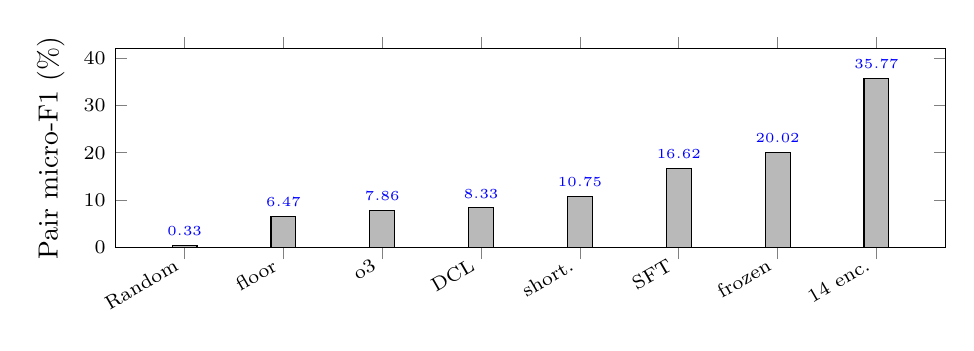
\begin{tikzpicture}
\begin{axis}[ybar,width=\columnwidth,height=4.1cm,bar width=9pt,ymin=0,ymax=42,ylabel={Pair micro-F1 (\%)},symbolic x coords={1,2,3,4,5,6,7,8},
 xtick=data,xticklabels={Random,floor,o3,DCL,short.,SFT,frozen,14 enc.},tick label style={font=\scriptsize},nodes near coords,nodes near coords style={font=\tiny},x tick label style={rotate=30,anchor=east}]
\addplot+[fill=gray!55,draw=black] coordinates {(1,0.33) (2,6.47) (3,7.86) (4,8.33) (5,10.75) (6,16.62) (7,20.02) (8,35.77)};
\end{axis}
\end{tikzpicture}
\caption{AEGIS-Bench, authors' file: published rows (Random, o3, DCL, Aegis-SFT), our trivial floor, shortcut-only (no text), frozen-encoder model and the 14-encoder ensemble}
\label{fig:aegis}
\end{figure}

\subsection{Reproduction check of lighter baselines}\label{sec:repro}
To test whether our pipeline and the published rows are comparable at all, we ran the two published baselines that fit our compute (Table~\ref{tab:repro}). The table also lists our own floor, frequency, flat-MLP and shortcut-only rows, so every row we ran uses the same test records and the authors' scorer. These are a check, not a replacement for the published rows.

\textbf{Qwen2.5-7B zero-shot.} We ran the model on the Hugging Face file and Who\&When with the authors' prompt (AWQ 4-bit weights, greedy decoding, 512 new tokens, long prompts cut to the first 30\% and last 70\% of the budget; 8 of 600 outputs unparseable and counted as empty). Pair and error micro-F1 are of the same size as the published row (pair \rpQwPair{} against \pubQwPair, error \rpQwError{} against \pubQwError{}), and so are the Who\&When pair and error values (pair \rpQwWWpair{} against 2.31, error \rpQwWWerror{} against 3.64). Agent-level micro-F1 on the AEGIS file is \emph{not} reproduced: \rpQwAgent{} against \pubQwAgent{} published, and our value is itself below the trivial floor of \floorHFagent{}. We did not isolate the cause; candidates are the test file (the published one is not named), 4-bit weights, the prompt variant, sampling against greedy decoding, and the rule for unparseable outputs.

\textbf{DCL-style.} No DCL code or checkpoint is released, so we re-implemented the published design with a frozen encoder (agent and mode prototype banks, top-$K$ pooling, asymmetric, contrastive and hierarchical losses) and trained it under the deduplicated protocol. It is a different model, and we name it DCL-style. On the authors' file it scores \rpDclPair{} pair micro-F1 (\rpDclPairLo--\rpDclPairHi), above the published DCL (\pubDCL) and below the all-blocks ensemble (\ensAEpair). The agent-level gap is large: \rpDclAgent{} against \pubDCLagent{} published, with a trivial floor of \floorAEagent{}. On Who\&When it gets pair \rpDclWWpair{}, agent \rpDclWWagent{} and error \rpDclWWerror{}, against \pubDCLwwPair{}, \pubDCLwwAgent{} and \pubDCLwwError{} published.

\textbf{What this shows.} Published pair and error micro-F1 can be approached or exceeded by simple models, in line with Section~\ref{sec:shortcut}. Published agent-level rows cannot be matched or bracketed by any model we ran, and they lie far below the trivial floor, so we do not use the agent-level rows of weaker methods as evidence about those methods. At pair level the rows we ran order as expected: zero-shot Qwen2.5-7B (\rpQwPair{} on the Hugging Face file), the no-text model (\shortAEpair{} on the authors' file), DCL-style (\rpDclPair), then the ensemble (\ensAEpair). A text-reading supervised model is thus only about two points above the no-text model, and the ensemble's gain comes mostly from fine-tuning.

\begin{table*}[t]
\caption{Reproduction check (micro-F1, \%). Rows marked ``rep.'' are copied from Table~1 of~\cite{aegis}; every row marked ``ours'' was run by us, scored with the authors' scorer on the same test records and with 95\% record-level intervals. The last four rows (trivial floor, frequency, flat MLP, shortcut-only MLP) use the same deduplicated training data as the ensemble; the flat MLP and shortcut-only MLP use frozen embeddings and five head seeds. Qwen2.5-7B (zero-shot, AWQ 4-bit, greedy, long prompts truncated) was run on the Hugging Face file only. DCL-style is our frozen-encoder re-implementation of the published design, trained under the deduplicated protocol (5 seeds), and is not the published DCL. Frequency scores zero on Who\&When because it predicts agent names seen in training, and Who\&When agent names are free-form. The published rows were evaluated on a test file the paper does not name.}
\label{tab:repro}
\centering\footnotesize\setlength{\tabcolsep}{3pt}
\begin{lrbox}{\fitbox}\begin{tabular}{@{}llrrrrrr@{}}
\toprule
 & & \multicolumn{3}{c}{AEGIS-Bench test file} & \multicolumn{3}{c}{Who\&When} \\
\cmidrule(lr){3-5}\cmidrule(lr){6-8}
Model & Test file & Pair & Agent & Error & Pair & Agent & Error \\
\midrule
Qwen2.5-7B, rep. & unnamed & 5.02 & 27.55 & 14.96 & 2.31 & 40.92 & 3.64 \\
Qwen2.5-7B, ours & HF & 8.01 {\scriptsize[6.8, 9.3]} & 49.24 {\scriptsize[45.8, 52.5]} & 20.15 {\scriptsize[18.2, 22.2]} & 2.98 {\scriptsize[0.6, 5.5]} & 35.16 {\scriptsize[27.9, 42.1]} & 6.23 {\scriptsize[2.8, 9.9]} \\
\midrule
DCL, rep. & unnamed & 8.33 & 22.93 & 24.73 & 1.60 & 8.40 & 14.67 \\
DCL-style, ours & authors' & 12.64 {\scriptsize[11.6, 13.7]} & 63.64 {\scriptsize[61.1, 66.1]} & 30.88 {\scriptsize[29.4, 32.3]} & 3.01 {\scriptsize[1.8, 4.3]} & 38.12 {\scriptsize[34.0, 42.4]} & 11.02 {\scriptsize[8.7, 13.5]} \\
DCL-style, ours & HF & 13.90 {\scriptsize[13.0, 14.8]} & 69.42 {\scriptsize[67.9, 70.9]} & 32.89 {\scriptsize[31.4, 34.4]} & -- \\
\midrule
Trivial floor, ours & authors' & 6.47 {\scriptsize[6.2, 6.7]} & 62.00 {\scriptsize[59.7, 64.3]} & 26.19 {\scriptsize[25.4, 27.0]} & 3.42 {\scriptsize[3.1, 3.8]} & 38.32 {\scriptsize[35.0, 41.8]} & 13.33 {\scriptsize[13.3, 13.3]} \\
Frequency, ours & authors' & 10.77 {\scriptsize[10.0, 11.5]} & 69.55 {\scriptsize[66.7, 72.2]} & 27.24 {\scriptsize[26.3, 28.2]} & 0.00 {\scriptsize[0.0, 0.0]} & 0.00 {\scriptsize[0.0, 0.0]} & 0.00 {\scriptsize[0.0, 0.0]} \\
Flat MLP, frozen MiniLM, ours & authors' & 20.02 {\scriptsize[18.5, 21.5]} & 68.45 {\scriptsize[65.6, 71.0]} & 31.43 {\scriptsize[29.7, 33.0]} & 1.96 {\scriptsize[1.0, 3.1]} & 33.88 {\scriptsize[29.0, 39.2]} & 7.63 {\scriptsize[5.6, 10.0]} \\
Shortcut-only MLP, ours & authors' & 10.75 {\scriptsize[9.2, 12.4]} & 58.35 {\scriptsize[55.5, 61.2]} & 23.54 {\scriptsize[21.5, 25.7]} & 4.95 {\scriptsize[2.7, 7.5]} & 38.08 {\scriptsize[33.2, 43.0]} & 10.87 {\scriptsize[7.5, 14.7]} \\
\bottomrule
\end{tabular}\end{lrbox}\fitfinish
\end{table*}

\subsection{Where the ensemble does well}
Table~\ref{tab:breakdown} breaks the ensemble's authors'-file results down by benchmark and framework. Pair micro-F1 is between 32 and 46 on five of the six task families and on four of the six frameworks. Two groups are weak: the 60 SmolAgents records on GAIA reach only 6.5 pair and 8.1 error micro-F1, close to the trivial floor of \floorAE, and the 87 DyLAN records have an agent micro-F1 of 33.3 against 57 to 90 elsewhere, largely the name-format effect of Section~\ref{sec:names}. The headline score is an average over very uneven groups. The table uses one head seed and has no intervals, and groups of 40 to 60 records are noisy, so treat it as a pointer rather than a ranking.

\begin{table}[t]
\caption{Where the 14-encoder ensemble does well: micro-F1 (\%) on the authors' test file by benchmark and by framework (head seed 0, all blocks; one prediction per record, no intervals, so small groups are noisy).}
\label{tab:breakdown}
\centering\footnotesize\setlength{\tabcolsep}{3pt}
\begin{lrbox}{\fitbox}\begin{tabular}{@{}llrrrr@{}}
\toprule
Group & Value & $n$ & Pair & Agent & Error \\
\midrule
benchmark & GSM8K & 100 & 38.4 & 68.1 & 57.3 \\
benchmark & HumanEval & 100 & 32.4 & 66.0 & 46.2 \\
benchmark & MATH & 100 & 41.5 & 81.7 & 47.9 \\
benchmark & MMLU & 100 & 40.0 & 81.7 & 48.6 \\
benchmark & SciBench & 100 & 34.1 & 66.5 & 48.9 \\
benchmark & magentic+gaia & 40 & 46.2 & 81.9 & 48.4 \\
benchmark & smol+gaia & 60 & 6.5 & 56.7 & 8.1 \\
framework & agentverse & 117 & 41.9 & 89.6 & 50.8 \\
framework & dylan & 87 & 19.1 & 33.3 & 50.0 \\
framework & llm debate & 140 & 43.2 & 79.7 & 45.4 \\
framework & macnet & 156 & 39.2 & 76.6 & 50.7 \\
framework & magentic one & 40 & 46.2 & 81.9 & 48.4 \\
framework & smoagents & 60 & 6.5 & 56.7 & 8.1 \\
\bottomrule
\end{tabular}\end{lrbox}\fitfinish
\end{table}

\subsection{Which failure modes are hard}
Table~\ref{tab:permode} gives pair-level scores per failure mode, from 67.4 F1 for FM-1.3 down to 10.1 for FM-3.3, with FM-1.4 (18.1) and FM-2.5 (15.5) also low. This fits the oracle diagnostic (Table~\ref{tab:oracle}), where knowing the true modes raised pair F1 far more than knowing the true agents. It also bears on transfer: FM-3.3 is the weakest mode in-domain yet makes up about 21\% of Who\&When labels, and FM-2.6 (26.7 F1 here) about 26\%. A model that is weakest on the modes that dominate natural data may transfer badly whatever we do to the mode prior. We did not test this directly, so it is a possible contributor, not an established cause.

\begin{table}[t]
\caption{Per failure mode, pair level: gold and predicted counts, precision, recall and F1 (\%) of the ensemble on the authors' file (head seed 0, all blocks). A pair counts as correct only if agent and mode both match.}
\label{tab:permode}
\centering\footnotesize\setlength{\tabcolsep}{3pt}
\begin{lrbox}{\fitbox}\begin{tabular}{@{}lrrrrr@{}}
\toprule
Mode & Gold & Pred. & Prec. & Rec. & F1 \\
\midrule
FM-1.1 & 155 & 219 & 39.7 & 56.1 & 46.5 \\
FM-1.2 & 83 & 103 & 35.9 & 44.6 & 39.8 \\
FM-1.3 & 94 & 93 & 67.7 & 67.0 & 67.4 \\
FM-1.4 & 95 & 71 & 21.1 & 15.8 & 18.1 \\
FM-1.5 & 92 & 152 & 25.7 & 42.4 & 32.0 \\
FM-2.1 & 83 & 104 & 25.0 & 31.3 & 27.8 \\
FM-2.2 & 117 & 100 & 52.0 & 44.4 & 47.9 \\
FM-2.3 & 102 & 100 & 54.0 & 52.9 & 53.5 \\
FM-2.4 & 87 & 135 & 29.6 & 46.0 & 36.0 \\
FM-2.5 & 71 & 122 & 12.3 & 21.1 & 15.5 \\
FM-2.6 & 98 & 119 & 24.4 & 29.6 & 26.7 \\
FM-3.1 & 90 & 117 & 27.4 & 35.6 & 30.9 \\
FM-3.2 & 116 & 105 & 33.3 & 30.2 & 31.7 \\
FM-3.3 & 46 & 53 & 9.4 & 10.9 & 10.1 \\
\bottomrule
\end{tabular}\end{lrbox}\fitfinish
\end{table}

\section{Transfer to Who\&When}\label{sec:ww}
Table~\ref{tab:ww} gives the results on 184 natural failures. The frozen model with all blocks scores \wwFullPair{} pair micro-F1, at or below the floor (\floorWW), while the shortcut-only model scores \wwShortPair. The fine-tuned ensemble with all blocks reaches \wwAllNo{} (\wwAllNoLo--\wwAllNoHi), whose interval overlaps the shortcut-only model's. The published o3 row is \pubOthreeWW{} pair and \pubOthreeWWagent{} agent micro-F1.

\subsection{Block masks and label shift (exploratory)}
Table~\ref{tab:gridci}, Fig.~\ref{fig:ww} and Table~\ref{tab:shiftgain} vary which blocks are visible. Label shift with all blocks on changes pair micro-F1 from \wwAllNo{} to \wwAllShift{} (paired gain \sgDdOO{}, interval \sgDdOOLo{} to \sgDdOOHi{}), not distinguishable from zero. With the name block on and the peer block off, shift raises it from \wwNameNo{} to \wwNameShift{} (paired gain \sgDdOF{}, interval \sgDdOFLo{} to \sgDdOFHi{}, the only mask whose interval excludes zero) and error micro-F1 to \wwNameShiftErr. With both blocks off the gain is \sgDdFF{} (\sgDdFFLo{} to \sgDdFFHi{}) and depends on the head seed; with names hidden and the peer block on it is \sgDdFO{} (\sgDdFOLo{} to \sgDdFOHi{}). We chose the name-on/peer-off mask after seeing Who\&When, so it is an exploratory lead, not a headline. A leave-one-framework-out check (Table~\ref{tab:lofo}; three encoders, one head seed) did not separate the masks beyond noise (all blocks on 18.16 against 17.44 to 17.74 pair), and it ran after all four masks had been scored, so it does not justify the choice. Agent micro-F1 with all blocks is \wwAllAgent, below the published o3 row (\pubOthreeWWagent).

\begin{figure}[t]
\centering
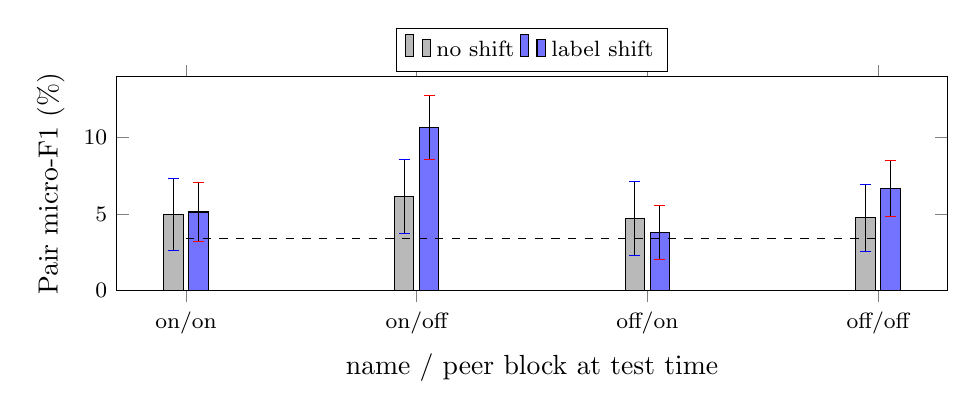
\begin{tikzpicture}
\begin{axis}[ybar,width=\columnwidth,height=4.3cm,bar width=7pt,ymin=0,ymax=14,ylabel={Pair micro-F1 (\%)},
 symbolic x coords={1,2,3,4},xtick=data,xticklabels={on/on,on/off,off/on,off/off},xlabel={name / peer block at test time},
 legend style={at={(0.5,1.02)},anchor=south,legend columns=3,font=\footnotesize},tick label style={font=\footnotesize},
 error bars/y dir=both,error bars/y explicit]
\addplot+[fill=gray!55,draw=black] coordinates {(1,4.96) +- (0,2.35) (2,6.16) +- (0,2.43) (3,4.71) +- (0,2.44) (4,4.77) +- (0,2.19)};
\addplot+[fill=blue!55,draw=black] coordinates {(1,5.14) +- (0,1.91) (2,10.68) +- (0,2.09) (3,3.78) +- (0,1.76) (4,6.67) +- (0,1.84)};
\draw[dashed] (axis cs:1,3.42) -- (axis cs:4,3.42);
\legend{no shift,label shift,trivial floor}
\end{axis}
\end{tikzpicture}
\caption{Who\&When pair micro-F1 of the 14-encoder ensemble by test-time block mask, with and without label shift (bars: 95\% intervals; dashed: trivial floor). Shift helped clearly only with the name block on and the peer block hidden (Table~\ref{tab:shiftgain})}
\label{fig:ww}
\end{figure}

\subsection{Relation to the earlier study}
The earlier query-disjoint study (Table~\ref{tab:legacygrid}) found that shift raised the all-blocks ensemble from 5.56 to 8.24 pair micro-F1. Table~\ref{tab:shiftgain} compares the paired gains of three configurations on the same 184 records. For all blocks the gain was \sgOldOO{} (\sgOldOOLo{} to \sgOldOOHi{}) in the earlier study, \sgFullOO{} (\sgFullOOLo{} to \sgFullOOHi{}) with the same encoders and heads trained on the full released split with duplicates, and \sgDdOO{} (\sgDdOOLo{} to \sgDdOOHi{}) with the newly fine-tuned deduplicated encoders. The deduplicated gain is smaller than the earlier one by \sdOldOO{} (\sdOldOOLo{} to \sdOldOOHi{}), an interval that excludes zero, but not distinguishably smaller than the full-released one (\sdFullOO{}, \sdFullOOLo{} to \sdFullOOHi{}). For the name-on/peer-off mask the comparison goes the other way: the deduplicated gain is larger than the earlier one by \sdOldOF{} (\sdOldOFLo{} to \sdOldOFHi{}, excluding zero) and not distinguishably different from the full-released one (\sdFullOF{}, \sdFullOFLo{} to \sdFullOFHi{}). The configurations differ in encoder fine-tuning data (3,234 gradient-update and 631 early-stopping records against 5,844 and 1,068), in head and threshold data (3,865 and 940 records against 6,912 and 1,657) and in the exported vectors. We cannot say which difference matters, since the old encoder vectors are no longer available. We therefore do not claim that label shift helps in general: its effect depends on the configuration.

\begin{table*}[t]
\caption{Effect of label shift on Who\&When pair micro-F1 (shift minus no shift, percentage points) by protocol and block mask, with paired 95\% record-level bootstrap intervals (10,000 resamples of the 184 records, 3 head seeds pooled). Bold: interval excludes zero. ``Earlier'': 14 encoders and heads trained on the 3,865 query-disjoint records. ``Full released'': the same old encoders with heads trained on the full released split (7,146 records, duplicates included). ``Dedup.'': the 14 newly fine-tuned encoders of the deduplicated protocol. All shift rows are transductive.}
\label{tab:shiftgain}
\centering\footnotesize\setlength{\tabcolsep}{3pt}
\begin{lrbox}{\fitbox}\begin{tabular}{@{}lcccc@{}}
\toprule
Protocol & on / on & on / off & off / on & off / off \\
\midrule
Earlier (query-disjoint) & \textbf{+2.68 {\scriptsize[+0.19, +5.04]}} & +1.32 {\scriptsize[-0.34, +2.93]} & \textbf{-1.63 {\scriptsize[-3.36, -0.12]}} & -1.09 {\scriptsize[-2.51, +0.26]} \\
Full released (duplicates) & +1.64 {\scriptsize[-1.44, +4.63]} & +2.40 {\scriptsize[-0.42, +5.24]} & +0.95 {\scriptsize[-1.12, +2.95]} & \textbf{+2.46 {\scriptsize[+0.39, +4.58]}} \\
Dedup. (this paper) & +0.19 {\scriptsize[-1.56, +1.88]} & \textbf{+4.51 {\scriptsize[+1.78, +7.22]}} & -0.93 {\scriptsize[-3.05, +1.16]} & +1.91 {\scriptsize[-0.16, +3.92]} \\
\midrule
Dedup. minus earlier & -2.49 {\scriptsize[-4.65, -0.22]} & +3.20 {\scriptsize[+0.59, +5.92]} & -- & -- \\
Dedup. minus full released & -1.45 {\scriptsize[-4.70, +1.77]} & +2.12 {\scriptsize[-0.71, +5.01]} & -- & -- \\
\bottomrule
\end{tabular}\end{lrbox}\fitfinish
\end{table*}

\section{Robustness, Sensitivity and Cost}\label{sec:robust}
The record-level intervals above ignore head-seed variation and do not test the gaps formally, and the headline rows use a single threshold rule. Here we add those checks, working from the saved ensemble probabilities (three head seeds, 14 encoders). None of them changes a headline number.

\textbf{Head-seed variability.} Table~\ref{tab:seedsd} gives mean and SD over the three head seeds. In-domain the spread is small (pair SD \sdAEpair{} on the authors' file). On Who\&When it is larger, \sdWWallPair{} points for the all-blocks row and \sdWWnameShiftPair{} for the name-on/peer-off row with shift, which is comparable to the gaps between masks. Three head seeds are few, and each encoder was trained once, so these SDs understate total variation.

\begin{table}[t]
\caption{Head-seed variability: mean $\pm$ SD over the three head seeds of the 14-encoder ensemble (micro-F1, \%). Block masks are name / peer (on or off). Shift rows are transductive and use Who\&When inputs only.}
\label{tab:seedsd}
\centering\footnotesize\setlength{\tabcolsep}{3pt}
\begin{lrbox}{\fitbox}\begin{tabular}{@{}llrrr@{}}
\toprule
Test set, mask & Shift & Pair & Agent & Error \\
\midrule
Authors' file, on / on & no & 35.77 $\pm$ 0.20 & 73.20 $\pm$ 0.41 & 45.79 $\pm$ 0.71 \\
HF file, on / on & no & 39.72 $\pm$ 0.41 & 84.31 $\pm$ 0.42 & 47.58 $\pm$ 0.77 \\
Who\&When, on / on & no & 4.96 $\pm$ 1.12 & 49.93 $\pm$ 0.64 & 7.96 $\pm$ 1.00 \\
Who\&When, on / off & no & 6.16 $\pm$ 0.46 & 51.03 $\pm$ 1.74 & 12.56 $\pm$ 1.56 \\
Who\&When, off / on & no & 4.71 $\pm$ 0.56 & 45.21 $\pm$ 0.63 & 7.90 $\pm$ 1.15 \\
Who\&When, off / off & no & 4.77 $\pm$ 0.76 & 46.19 $\pm$ 1.30 & 9.82 $\pm$ 1.51 \\
Who\&When, on / on & yes & 5.14 $\pm$ 1.97 & 51.69 $\pm$ 0.36 & 10.28 $\pm$ 5.24 \\
Who\&When, on / off & yes & 10.68 $\pm$ 2.18 & 51.27 $\pm$ 2.25 & 23.12 $\pm$ 3.72 \\
\bottomrule
\end{tabular}\end{lrbox}\fitfinish
\end{table}

\textbf{Paired tests.} Table~\ref{tab:paired} compares configurations on identical records. In-domain, using both blocks beats hiding both by \ptAEallNeither{} pair points (\ptAEallNeitherLo{} to \ptAEallNeitherHi) and beats hiding only the name block by \ptAEallNames, so name and peer features carry real in-domain signal; the difference to hiding only the peer block is not distinguishable from zero. On Who\&When, no pair of masks without shift differs reliably. Shift changes the name-on/peer-off mask by \sgDdOF{} (Wilcoxon $p$ \ptWWnameShiftP) and is indistinguishable from zero for the other three. That mask with shift is above the all-blocks no-shift row by \ptWWnameShiftVsAll{} (\ptWWnameShiftVsAllLo{} to \ptWWnameShiftVsAllHi). The bootstrap and Wilcoxon tests agree throughout. The ten comparisons were chosen after the masks had been scored and the mask itself was chosen post hoc, so these $p$-values do not make the result confirmatory, even though its $p$-value clears a Bonferroni level for ten tests.

\begin{table*}[t]
\caption{Paired tests on the same records (pair micro-F1 difference, percentage points; 10,000-resample record-level bootstrap interval; two-sided Wilcoxon signed-rank test on per-record pair F1 averaged over head seeds). Authors' file: 600 records; Who\&When: 184. Ten tests are shown, so a Bonferroni level is 0.005.}
\label{tab:paired}
\centering\footnotesize\setlength{\tabcolsep}{3pt}
\begin{lrbox}{\fitbox}\begin{tabular}{@{}lrr@{}}
\toprule
Comparison & Difference [95\% interval] & Wilcoxon $p$ \\
\midrule
Authors' file: on/on minus off/off & \textbf{+3.93 {\scriptsize[+2.54, +5.34]}} & $<$0.001 \\
Authors' file: on/on minus off/on & \textbf{+3.00 {\scriptsize[+1.93, +4.11]}} & $<$0.001 \\
Authors' file: on/on minus on/off & +0.84 {\scriptsize[-0.05, +1.78]} & 0.212 \\
Who\&W.: on/on minus off/off, no shift & +0.19 {\scriptsize[-1.51, +1.94]} & 0.575 \\
Who\&W.: shift minus no shift, on/on & +0.19 {\scriptsize[-1.51, +1.84]} & 0.566 \\
Who\&W.: shift minus no shift, on/off & \textbf{+4.51 {\scriptsize[+1.71, +7.25]}} & $<$0.001 \\
Who\&W.: shift minus no shift, off/on & -0.93 {\scriptsize[-3.07, +1.07]} & 0.289 \\
Who\&W.: shift minus no shift, off/off & +1.91 {\scriptsize[-0.18, +3.88]} & 0.190 \\
Who\&W.: on/off + shift minus on/on no shift & \textbf{+5.72 {\scriptsize[+2.74, +8.58]}} & $<$0.001 \\
Who\&W.: on/off + shift minus off/off no shift & \textbf{+5.91 {\scriptsize[+3.29, +8.48]}} & $<$0.001 \\
\bottomrule
\end{tabular}\end{lrbox}\fitfinish
\end{table*}

\textbf{Query-cluster intervals.} Conversations built from the same query are correlated, and Xu and Gao~\cite{audit2} resample query groups. Resampling the \clAEgroups{} query groups of the authors' file for the all-blocks ensemble gives a pair micro-F1 interval of \clAEpairLo--\clAEpairHi{} against \ensAEpairLo--\ensAEpairHi{} at record level, and the agent and error intervals move by 0.2 points or less, so the record-level intervals are not too narrow for this file. On Who\&When the two agree to 0.2 points.

\textbf{Threshold sensitivity.} Table~\ref{tab:sens} multiplies both tuned thresholds by a common factor. In-domain, pair micro-F1 on the authors' file stays within about two and a half points of the tuned value (at least \sensAEmin) for factors 0.75 to 1.5, and drops to \sensAEhalf{} at 0.5, where the decoder fires too often. On Who\&When the no-shift rows move by about one point or less over 0.75 to 1.5, and the shifted name-on/peer-off row stays between \sensShiftMin{} and \sensShiftMax{} over the whole range, so its gain over the unshifted rows is not an artefact of one threshold setting. The label-shift weights themselves were not varied.

\begin{table}[t]
\caption{Sensitivity of pair micro-F1 (\%) to the decision thresholds. Both tuned thresholds $(t_a, t_m)$ are multiplied by the same factor (1.0 is the tuned setting). Mean over three head seeds.}
\label{tab:sens}
\centering\footnotesize\setlength{\tabcolsep}{3pt}
\begin{lrbox}{\fitbox}\begin{tabular}{@{}lccccc@{}}
\toprule
Setting & 0.5 & 0.75 & 1.0 & 1.25 & 1.5 \\
\midrule
Authors' file, on / on & 28.33 & 33.40 & 35.77 & 35.54 & 35.01 \\
HF file, on / on & 32.94 & 37.62 & 39.72 & 39.53 & 38.99 \\
Who\&W., on / on & 4.99 & 5.09 & 4.96 & 4.74 & 4.69 \\
Who\&W., on / off & 7.06 & 6.45 & 6.16 & 5.78 & 5.40 \\
Who\&W., on / off + shift & 10.69 & 10.55 & 10.68 & 10.34 & 10.26 \\
\bottomrule
\end{tabular}\end{lrbox}\fitfinish
\end{table}

\textbf{Ensemble size and cost.} Table~\ref{tab:ensize} rebuilds the ensemble from the first $k$ encoders. A single fine-tuned encoder reaches \ensSingleAE{} $\pm$ \ensSingleAEsd{} pair micro-F1 on the authors' file, and the 14-encoder ensemble \ensKfourteenAE{}, with \ensKtwoAE{}, \ensKfourAE{} and \ensKsevenAE{} for $k=2,4,7$, so the ensemble is worth a few points and most of the gain over the frozen model (\fullAEdedup) comes from fine-tuning. On Who\&When the single-encoder score of the name-on/peer-off row with shift is \ensSingleWWshift{} $\pm$ \ensSingleWWshiftSd{} against \ensFourteenWWshift{} for 14 encoders. On a laptop CPU (Apple M5), building features for one encoder takes about \costFeat{} s and training the heads (three seeds, four masks, \costParams{} parameters each) about \costHead{} s; running all four masks on the validation, authors' and Who\&When rows takes about \costInf{} s per encoder. Fine-tuning one encoder on a free T4 takes about 222 s per epoch (Section~\ref{sec:methods}). The no-text baseline needs no fine-tuning and trains in seconds.

\begin{table}[t]
\caption{Ensemble size. Pair micro-F1 (\%), mean over three head seeds, when the ensemble is built from the first $k$ of the 14 fine-tuned encoders (``single'': mean $\pm$ SD, over the 14 encoders used alone). Thresholds are re-tuned on validation for each $k$.}
\label{tab:ensize}
\centering\footnotesize\setlength{\tabcolsep}{2pt}
\begin{lrbox}{\fitbox}\begin{tabular}{@{}lcccccc@{}}
\toprule
Setting & single & $k{=}1$ & 2 & 4 & 7 & 14 \\
\midrule
Authors' file, on / on & 31.66 $\pm$ 0.45 & 32.42 & 33.79 & 35.07 & 35.34 & 35.77 \\
Who\&W., on / off + shift & 9.73 $\pm$ 1.35 & 8.12 & 9.14 & 11.09 & 11.80 & 10.68 \\
\bottomrule
\end{tabular}\end{lrbox}\fitfinish
\end{table}

\section{Failure Case Studies}\label{sec:cases}
To see what hides behind the averages, we read individual records from the seed-0 ensemble: some from the authors' file (all blocks, no shift) and some from Who\&When (name-on/peer-off, with shift). We picked them to illustrate the patterns below; they are not a random sample.

\textbf{Right agent, wrong mode.} On Who\&When 139 of 184 records have the correct faulty agent among the predicted agents, yet 138 have no correct (agent, mode) pair and only two are exact. For example, \texttt{PythonDebugging\_Expert} is the gold agent with FM-2.2 in one record, and the model predicts that agent with FM-1.3, FM-2.6, FM-3.1 and FM-3.3 but not FM-2.2. An AgentVerse record on GSM8K (eight turns) has three faulty agents with FM-1.3, FM-1.5 and FM-3.3; the model finds all three agents and the first mode, and misses the other two (FM-1.4 for FM-1.5 and FM-2.5 for FM-3.3). This agrees with the oracle diagnostic of Section~\ref{sec:legacy}: pair F1 is limited mainly by mode choice, less by agent choice.

\textbf{Over-prediction on natural logs.} In another Who\&When record the gold is one agent (\texttt{Tickets\_Pricing\_Expert}) with FM-3.3; the model names a different agent (\texttt{Budgeting\_Expert}) with three modes (FM-1.3, FM-3.1, FM-3.3). The decoder emits every pair above its thresholds, so one wrong agent produces several false positives at once. The headline decoder does not exploit the fact that each Who\&When record has a single faulty agent.

\textbf{Long agentic logs.} The weakest group, SmolAgents on GAIA (60 records, 6.5 pair micro-F1), has long records. One has 31 turns whose first turn is a long system prompt, and the model predicts the right agent (\texttt{Searcher}) with FM-1.2 where the gold mode is FM-2.4. Each turn is cut to 256 tokens before embedding, so a system prompt can take the whole window; we did not test truncation as the cause.

\textbf{Scoring artefact.} In a DyLAN record on GSM8K the model predicts four pairs with the speakers' names (\texttt{Assistant1} to \texttt{Assistant4}) and the gold labels carry the lowercase names; all four pairs match after normalisation, and the exact-match score for this record is zero. This is the pattern behind Section~\ref{sec:names}: the authors' file can mark a correct prediction as wrong.

\section{Earlier Study on a Query-Disjoint Split (as Logged)}\label{sec:legacy}
Before the deduplicated-protocol work, we trained on a query-disjoint split. Every training and validation record whose query appears in the test set was dropped (4,128 of 8,933), which left 3,865 training and 940 validation records. These runs were scored on the Hugging Face test file and we did not repeat them for this paper, so Tables~\ref{tab:qd}--\ref{tab:oracle} are reported as logged. The judge rows were re-checked against their saved result files. For a frozen-encoder MLP, Table~\ref{tab:qd} shows validation pair F1 falling from 32.19 to 23.05 and test pair F1 from 33.08 to 19.83 under this split.

% Numbers in this file come from the earlier query-disjoint study (draft Tables III, VII-XIV), as logged on Kaggle and in the project ledger.
% They were NOT re-run for this paper. The k=5 and k=12 judge rows were re-checked against aegis/results/rr/final_rrf1.json and rr_k12/final_rrf2.json.

\begin{table}[t]
\caption{Earlier study, query-disjoint training split: frozen-encoder MLP, pair micro-F1 (\%), AEGIS validation and Hugging Face test file (as logged).}
\label{tab:qd}
\centering\footnotesize\setlength{\tabcolsep}{3pt}
\begin{lrbox}{\fitbox}\begin{tabular}{@{}lccc@{}}
\toprule
Training split & Train / val records & Val pair & Test pair \\
\midrule
Released split & 7,146 / 1,787 & 32.19 & 33.08 \\
Query-disjoint & 3,865 / 940 & 23.05 & 19.83 \\
\bottomrule
\end{tabular}\end{lrbox}\fitfinish
\end{table}

\begin{table*}[t]
\caption{Earlier study (query-disjoint, as logged): test-time block mask grid for a 14-encoder ensemble, mean $\pm$ population standard deviation (ddof 0) over 3 head seeds, micro-F1 pair / agent / error; label shift is transductive. The all-blocks gain seen here (5.56 to 8.24) is smaller in the deduplicated ensemble (Table~\ref{tab:shiftgain}).}
\label{tab:legacygrid}
\centering\footnotesize\setlength{\tabcolsep}{3pt}
\begin{lrbox}{\fitbox}\begin{tabular}{@{}lccc@{}}
\toprule
Name / peer block & AEGIS test & Who\&When, no shift & Who\&When, label shift \\
\midrule
on / on & 32.96$\pm$0.66 / 79.37$\pm$0.86 / 40.95$\pm$0.86 & 5.56$\pm$0.74 / 43.75$\pm$0.05 / 11.76$\pm$0.63 & 8.24$\pm$1.19 / 47.72$\pm$1.05 / 17.12$\pm$1.37 \\
on / off & 27.90$\pm$3.16 / 81.41$\pm$2.04 / 38.44$\pm$0.40 & 6.94$\pm$0.90 / 44.69$\pm$1.69 / 16.12$\pm$1.50 & 8.26$\pm$0.36 / 45.55$\pm$0.76 / 17.71$\pm$1.80 \\
off / on & 31.22$\pm$0.89 / 72.21$\pm$0.94 / 40.28$\pm$1.13 & 3.35$\pm$0.93 / 40.55$\pm$1.22 / 7.63$\pm$1.16 & 1.72$\pm$1.15 / 44.52$\pm$3.54 / 5.01$\pm$3.60 \\
off / off & 25.24$\pm$0.45 / 76.07$\pm$0.78 / 38.32$\pm$0.30 & 3.17$\pm$0.65 / 41.75$\pm$0.97 / 9.91$\pm$2.02 & 2.09$\pm$1.48 / 42.24$\pm$0.87 / 5.65$\pm$3.78 \\
\bottomrule
\end{tabular}\end{lrbox}\fitfinish
\end{table*}

\begin{table}[t]
\caption{Earlier study: leave-one-framework-out inside AEGIS (mean over 6 held-out frameworks; micro-F1; encoders es\_s0 to es\_s2, one head seed; differences between masks are small).}
\label{tab:lofo}
\centering\footnotesize\setlength{\tabcolsep}{3pt}
\begin{lrbox}{\fitbox}\begin{tabular}{@{}lccc@{}}
\toprule
Mask (name / peer) & Pair & Agent & Error \\
\midrule
on / on & 18.16 & 70.56 & 26.75 \\
on / off & 17.44 & 69.76 & 26.75 \\
off / on & 17.74 & 62.90 & 27.57 \\
off / off & 17.62 & 63.42 & 29.89 \\
\bottomrule
\end{tabular}\end{lrbox}\fitfinish
\end{table}

\begin{table}[t]
\caption{Earlier study: framework-adversarial training on single encoders (AEGIS test pair; Who\&When pair / agent / error micro-F1; as logged).}
\label{tab:adv}
\centering\footnotesize\setlength{\tabcolsep}{3pt}
\begin{lrbox}{\fitbox}\begin{tabular}{@{}lcc@{}}
\toprule
Variant & AEGIS pair & Who\&When \\
\midrule
Reference (no adversary) & 27.80 & 5.13 / 41.00 / 14.00 \\
$\lambda=0.5$, seed 0 & 19.43 & 4.20 / 42.97 / 12.40 \\
$\lambda=0.5$, seed 1 & 19.90 & 3.50 / 42.37 / 13.00 \\
$\lambda=1.0$ & 19.40 & 4.57 / 42.83 / 13.70 \\
$\lambda=0.5$ + name-dropout & 19.40 & 4.60 / 41.33 / 12.53 \\
$\lambda=1.0$ + name-dropout & 19.07 & 4.17 / 38.77 / 14.77 \\
\bottomrule
\end{tabular}\end{lrbox}\fitfinish
\end{table}

\begin{table*}[t]
\caption{Earlier study: frozen Qwen2.5-7B judge with 95\% bootstrap intervals (pair micro-F1 unless stated). Differences are over the same records. Model alone is a 3-seed ensemble; the shortlist model is the pre-committed headline.}
\label{tab:judge}
\centering\footnotesize\setlength{\tabcolsep}{3pt}
\begin{lrbox}{\fitbox}\begin{tabular}{@{}llll@{}}
\toprule
Data & Row & Pair micro-F1 [95\% CI] & Paired difference vs model alone \\
\midrule
AEGIS test & Model alone & 34.02 [31.80, 36.37] & -- \\
AEGIS test & Shortlist model, $k{=}5$ & 33.57 [31.42, 35.75] & $-0.45$ [$-1.27$, $+0.37$] pair; $+1.28$ [$+0.51$, $+1.99$] agent \\
AEGIS test & Judge alone, plain, $k{=}5$ & 24.98 [23.01, 27.16] & $-9.04$ pair \\
AEGIS test & Judge alone, rag, $k{=}5$ & 27.00 [25.08, 29.15] & $-7.01$ pair \\
Who\&When & Model alone & 9.21 [6.99, 11.60] & -- \\
Who\&When & Shortlist model, $k{=}5$ & 8.96 [6.31, 11.66] & -- \\
Who\&When & Judge alone, plain, $k{=}5$ & 11.05 [8.34, 14.00] & $+1.82$ [$-0.19$, $+3.74$] pair; $+6.65$ [$+3.54$, $+9.88$] agent \\
Who\&When & Judge alone, rag, $k{=}5$ & 8.57 [6.09, 11.55] & -- \\
Who\&When (study 2) & Shortlist model, $k{=}12$ & 8.94 [6.50, 11.36] & $-0.29$ [$-1.52$, $+0.79$] pair \\
Who\&When (study 2) & Judge alone, plain, $k{=}12$ & 9.67 [7.96, 11.31] & $+0.41$ [$-1.67$, $+2.53$] pair; $+1.09$ [$-1.64$, $+3.72$] agent \\
\bottomrule
\end{tabular}\end{lrbox}\fitfinish
\end{table*}

\begin{table}[t]
\caption{Earlier study: shortlist recall of the trained model (\%), the share of gold pairs in the top-$k$ candidates.}
\label{tab:recall}
\centering\footnotesize\setlength{\tabcolsep}{3pt}
\begin{lrbox}{\fitbox}\begin{tabular}{@{}lcccc@{}}
\toprule
 & $k{=}1$ & $k{=}5$ & $k{=}8$ & $k{=}12$ \\
\midrule
AEGIS validation & 22.6 & 51.1 & 60.9 & 71.1 \\
Who\&When (diagnostic) & 1.6 & 28.8 & 42.9 & 52.7 \\
\bottomrule
\end{tabular}\end{lrbox}\fitfinish
\end{table}

\begin{table}[t]
\caption{Earlier study: oracle diagnostic on the AEGIS test file (single encoder, micro-F1; pair / agent / error).}
\label{tab:oracle}
\centering\footnotesize\setlength{\tabcolsep}{3pt}
\begin{lrbox}{\fitbox}\begin{tabular}{@{}lccc@{}}
\toprule
 & Pair & Agent & Error \\
\midrule
Model & 27.79 & 81.37 & 38.66 \\
Oracle agents & 31.12 & 92.20 & 40.09 \\
Oracle modes & 56.06 & 72.05 & 79.90 \\
\bottomrule
\end{tabular}\end{lrbox}\fitfinish
\end{table}

\begin{table*}[t]
\caption{Earlier study (query-disjoint, as logged), our rows with micro / macro F1 (\%) at pair, agent and error level. Who\&When rows are the mean over three head seeds; label shift is transductive. Dashes: not computed.}
\label{tab:legacymacro}
\centering\footnotesize\setlength{\tabcolsep}{3pt}
\begin{lrbox}{\fitbox}\begin{tabular}{@{}llcccccc@{}}
\toprule
Test set & Model & Pair mi & Pair ma & Agent mi & Agent ma & Error mi & Error ma \\
\midrule
AEGIS (HF file) & Trivial floor & 7.35 & 6.35 & 68.58 & 61.98 & 27.14 & 26.99 \\
AEGIS (HF file) & Frozen encoder, flat MLP & 19.83 & 12.99 & 78.74 & 65.27 & 33.01 & 32.62 \\
AEGIS (HF file) & Fine-tuned, all blocks (14 enc.) & 32.96 & 18.86 & 79.37 & 66.06 & 40.95 & 39.47 \\
Who\&When & Trivial floor & 3.42 & 2.85 & 38.32 & 38.41 & 13.33 & 12.34 \\
Who\&When & Frozen encoder, flat MLP & 4.25 & -- & 39.60 & -- & 10.83 & -- \\
Who\&When & Fine-tuned, all blocks, no shift & 5.56 & 3.14 & 43.75 & 32.07 & 11.76 & 7.86 \\
Who\&When & Fine-tuned, all blocks, label shift & 8.24 & 4.86 & 47.72 & 38.69 & 17.12 & 5.08 \\
\bottomrule
\end{tabular}\end{lrbox}\fitfinish
\end{table*}

\begin{table}[t]
\caption{Earlier study: name-dropout on single encoders (mean of 3 head seeds; AEGIS test pair, then Who\&When pair / agent / error micro-F1; as logged).}
\label{tab:namedrop}
\centering\footnotesize\setlength{\tabcolsep}{3pt}
\begin{lrbox}{\fitbox}\begin{tabular}{@{}llcc@{}}
\toprule
Encoder & Recipe & AEGIS pair & Who\&When \\
\midrule
s0 & Base & 27.80 & 5.13 / 41.00 / 14.00 \\
s0 & Name-dropout & 26.00 & 6.03 / 47.03 / 14.53 \\
s1 & Base & 27.73 & 6.07 / 41.27 / 16.60 \\
s1 & Name-dropout & 27.70 & 6.70 / 45.47 / 16.03 \\
7 enc. & Name-dropout & 26.88 & 6.80 / 45.78 / 16.12 \\
\bottomrule
\end{tabular}\end{lrbox}\fitfinish
\end{table}

\subsection{Micro and macro F1 together}
Table~\ref{tab:legacymacro} adds macro-F1 for the earlier study. Macro-F1 on Who\&When is weak for every system, ours included. Pair macro-F1 was above the floor (4.86 against 2.85 with label shift), but agent macro-F1 (32.07 without shift, 38.69 with) was at or below the floor's 38.41, and error macro-F1 (7.86 and 5.08) was well below the floor's 12.34. Label shift raised micro-F1 by pushing predictions toward the dominant natural modes, and it lowered macro error, so rare modes were not recovered. The two scores tell different stories and should be read together, which is why Table~\ref{tab:pubfull} lists both.

\subsection{Name-dropout on single encoders}
Table~\ref{tab:namedrop} shows name-dropout on single encoders. Hiding the name block raised Who\&When agent F1 by 4.2--6.0 points at a cost of 0--2 AEGIS pair points; the pair gain (+0.6 to +0.9) was inside seed noise. This is the earlier study's reason for the block-mask design of Section~\ref{sec:methods}.

\subsection{Framework-adversarial training (RQ5)}
Table~\ref{tab:adv} gives single-encoder results against non-adversarial encoders trained identically (AEGIS test pair 27.7--27.8, Who\&When pair 5.1--6.1). Adversarial training lowered AEGIS pair by 7--10 points and gave no Who\&When gain: Who\&When pair stayed at 3.5--4.6 and agent F1 at 38.8--43.0. A plausible explanation, which we did not test, is that framework style is correlated with the labels in AEGIS, so removing it also removes useful signal. The leave-one-framework-out results (Table~\ref{tab:lofo}) give no support for removing framework information.

\subsection{A frozen LLM judge (RQ5)}
Table~\ref{tab:judge} shows both judge studies. In study 1 ($k=5$) the shortlist passed its gate (recall at 5 of 51.1 against recall at 1 of 22.6 on AEGIS validation, a ratio of 2.26; Table~\ref{tab:recall}), but the judge alone scored 24.98 AEGIS pair against 34.02 for the trained ensemble, and retrieved in-domain examples raised it only to 27.00. All fusion weights tuned on AEGIS validation came out as 0, so the pre-committed headline reduced to the shortlist model. On Who\&When the judge alone gained 1.82 pair (95\% interval $-0.19$ to $+3.74$) and 6.65 agent points ($+3.54$ to $+9.88$) over the model, but this was one of eight post hoc contrasts. It did not replicate in the pre-registered study 2 with $k=12$: judge-alone minus model was $+0.41$ pair ($-1.67$ to $+2.53$), the tuned fusion weight was again 0, and the success bar was not met. A judge can only reorder candidates the model already proposed: on Who\&When recall at 5 is 28.8 and at 12 is 52.7, against a reachable share of 89.1. These findings hold for a 4-bit zero-shot 7B judge with at most about 7,000 prompt tokens; larger or API judges were not tested.

\subsection{Where the errors are}
An oracle diagnostic (Table~\ref{tab:oracle}) shows that choosing the mode is what holds pair F1 back. Handing the model the true faulty agents adds 3.3 points of pair F1; handing it the true modes adds 28.3. Of the faulty agents the model does find, it gets the exact mode set right only 21.2\% of the time. The oracle-mode figure uses trajectory-level truth, so it is an upper bound and not a target. It also explains why remedies that work on agent features mostly move agent F1.

\subsection{Zero-shot LLMs in-domain}
The published zero-shot rows (Table~\ref{tab:aegis}) sit near the trivial floor at pair level, and the published agent-level numbers sit below our agent floor. We report this as an observation without building a claim on it, since explaining published results is outside our scope.

\section{Discussion}
\subsection{Summary of research questions}
Table~\ref{tab:rq} summarises the outcome of each question.

\begin{table}[t]
\caption{Research questions and outcomes.}
\label{tab:rq}
\centering\footnotesize
\begin{tabularx}{\columnwidth}{@{}l l Y@{}}
\toprule
RQ & Outcome & Evidence \\
\midrule
RQ1 & Supported & Duplicates inflate pair micro-F1 by \dropAE--\dropHF{} points; shortcut-only \shortAEpair{} against floor \floorAE \\
RQ2 & Partly supported & Pair \ensAEpair{} and error \ensAEerror{} above published Aegis-SFT; agent \ensAEagent{} below \pubSFTagent \\
RQ3 & Large gap & \ensAEpair{} in-domain against \wwAllNo{} on Who\&W.; block masks stay within intervals of one another except one post hoc mask \\
RQ4 & Conditional & Shift gain \sgDdOF{} (paired interval excludes zero) with the peer block hidden (post hoc), \sgDdOO{} with all blocks; the pattern differs across training configurations \\
RQ5 & Not supported (earlier study) & Adversary lowers AEGIS pair by 7--10; judge adds nothing in two studies \\
\bottomrule
\end{tabularx}
\end{table}


The released AEGIS files contain verbatim duplicates, and a model that never reads the text already beats several published rows. A pair micro-F1 on AEGIS-Bench says little until it is put next to a trivial floor, a no-text baseline and a duplicate-free training set. Under that protocol the fine-tuned ensemble does well in-domain (pair \ensAEpair{} against \pubSFT{}). On natural failures it does no better than the no-text model, unless we hide the peer block and apply label shift, and we chose that combination after seeing the results.

\textbf{RQ1.} Two separate things sit in the released files. Overlap: shared queries between training and test are expected when several faulty variants are generated per task, but verbatim duplicate conversations let a model memorise. Shortcuts: agent name, framework and turn counts alone predict a useful share of the labels. The frozen model loses \dropAE{} points when duplicates are removed, and what remains is partly accounted for by the no-text baseline (\shortAEpair{} of \fullAEdedup). We do not claim either effect was intended, and we cannot say whether the published models were trained with the duplicates.

\textbf{RQ2.} The ensemble is better than the published rows at pair and error level and worse at agent level. Pair and error micro-F1 reward choosing the right modes, while agent micro-F1 rewards finding the faulty agent, where a 14B generative model has the advantage. The breakdown by group also shows that the average hides large differences, so one headline number is not enough for a tool used on one framework at a time.

\textbf{RQ3 and RQ4.} On natural failures the all-blocks ensemble sits at the level of the no-text model, and the gap between \ensAEpair{} in-domain and \wwAllNo{} on Who\&When is large however the intervals are read. Hiding the peer block and applying label shift gives the best Who\&When numbers we measured, including \wwNameShiftErr{} error micro-F1 against \pubOthreeWWerr{} for the published o3 row. We hold this result back for three reasons: the mask was chosen after seeing Who\&When, it is the only mask whose paired gain excludes zero, and the all-blocks gain of the earlier study (\sgOldOO{}) shrank in the deduplicated run (\sgDdOO{}). The safest reading is that the effect of label shift depends on how the model was trained, and we cannot yet say why.

Injected and natural failures may differ in ways our data are consistent with: agent names and roles are specific to each dataset, the mode mix is skewed in natural logs, and injected logs carry framework styles that the natural set lacks. Block masks and label shift address the first two directly. We did not test whether the injector artefacts discussed in~\cite{audit1,audit2} show up in our features.

Cost is modest. The trained attributor produces its output in minutes on a CPU from saved vectors, after a one-off fine-tune of about 222 s per epoch on a T4 GPU. Each judge pass in the earlier study took 3.4 to 4.1 hours on a Kaggle kernel and gave us nothing measurable. A cheap trained model with honest controls makes a useful baseline for this task, but it is no substitute for a stronger LLM.

If you only have injected data, we would suggest the following. Check the released splits for verbatim and query overlap. Report a trivial floor, a no-text baseline and record-level intervals beside every trained model. Hide feature blocks at random during training. And treat label shift as an exploratory, transductive step that still needs checking.

\textbf{Choosing a configuration.} Table~\ref{tab:choose} turns our results into a decision aid for these two benchmarks only; the Who\&When rows rest on 184 records.

\begin{table}[t]
\caption{Which configuration to use, by constraint (pair micro-F1, \%, from the tables above).}
\label{tab:choose}
\centering\footnotesize
\begin{tabularx}{\columnwidth}{@{}Y Y Y@{}}
\toprule
Constraint & Configuration & Evidence and caveat \\
\midrule
No GPU, seconds of compute & No-text shortcut model, or frozen MiniLM MLP & \shortAEpair{} and \fullAEdedup{} on the authors' file; use as baselines, not as attributors \\
One free-GPU session & One fine-tuned encoder, all blocks & \ensSingleAE{} $\pm$ \ensSingleAEsd{} on the authors' file (14 encoders used alone) \\
Best in-domain accuracy & 14-encoder ensemble, all blocks & \ensAEpair{} (\ensAEpairLo--\ensAEpairHi); a few points over a single encoder; weak on SmolAgents/GAIA \\
Natural failures, no target labels & No validated choice; all-blocks ensemble is at the shortcut level & \wwAllNo{} against \wwShortPair{}; name-on/peer-off with label shift reaches \wwNameShift{} but was chosen post hoc \\
Agent-level scoring on the authors' file & Report exact and name-normalised scores together & \nmAgentExact{} against \nmAgentNorm{} agent micro-F1 (Section~\ref{sec:names}) \\
One framework at a time & Check the per-framework breakdown first & Pair micro-F1 ranges from 6.5 to 46 across groups (Table~\ref{tab:breakdown}) \\
\bottomrule
\end{tabularx}
\end{table}

\textbf{A reporting checklist.} The audit suggests eight items that an attribution paper can report at little cost (Table~\ref{tab:check}). None needs new training; the first four need only the released files and a scorer.

\begin{table}[t]
\caption{Reporting checklist for failure-attribution results.}
\label{tab:check}
\centering\footnotesize
\begin{tabularx}{\columnwidth}{@{}l Y Y@{}}
\toprule
\# & Item & Why \\
\midrule
1 & Name the test file and its source & Two released files differ in benchmark mix \\
2 & Report verbatim and query overlap between all splits & \dupTrainPct\% of one released test file duplicates training records \\
3 & Report the trivial floor of the same file & Floors differ by file (\floorAE, \floorHF, \floorWW) \\
4 & Report a no-text baseline & Name, framework and counts alone reach \shortAEpair \\
5 & Verify the scorer against the authors' & Parity to $10^{-12}$ is checkable \\
6 & Report record-level intervals & Who\&When has 184 records \\
7 & Mark transductive and post hoc steps & Label shift reads target inputs; one mask was chosen post hoc \\
8 & Report all three levels and macro-F1 & Agent-level can fall below published rows while pair rises \\
\bottomrule
\end{tabularx}
\end{table}

\section{Threats to Validity and Limitations}\label{sec:limits}
\emph{Internal validity.} Head-seed spread is not part of the intervals, which are record-level; each fine-tuned encoder was trained once, and thresholds are global rather than per-mode. \emph{Construct validity.} Pair F1 on Who\&When depends on an LLM-based mapping of free-text reasons to 14 modes and on agent-name matching, so part of the measured error is annotation error. \emph{External validity.} One injected dataset, one natural dataset, one small encoder family.
\begin{enumerate}
\item Who\&When has 184 records and is a single natural test set; intervals are wide, and claims concern this benchmark only. Who\&When mode labels come from an LLM mapping, so error-level numbers are weaker evidence than agent-level numbers.
\item The peer-hidden label-shift result was selected after seeing Who\&When; the leave-one-framework-out check was run afterwards and did not separate the masks. Thresholds and early stopping use only AEGIS data. The three-seed intervals and the significance tests of Section~\ref{sec:robust} are paired over records but treat the head seeds as fixed, were run after the masks had been scored, and do not cover independently trained encoders.
\item Label shift is transductive, and its assumptions (calibration, stable $P(\text{text}\mid\text{mode})$) are untested for our model.
\item Published rows are copied as reported and were not reproduced; the published paper does not name its test file, so comparisons are against numbers on an unnamed file. We reproduced only two lighter baselines (Section~\ref{sec:repro}); the Qwen run used the Hugging Face file and a 4-bit model, DCL-style is not the published DCL, and we did not reproduce the 14B models or compare against other attribution methods (Section~\ref{sec:scope}).
\item Our novelty checks were limited to search results and to reading the related audits~\cite{audit1,audit2,catch} through a summarising tool (the first in full, the second in its main text, the third at abstract level). ``We did not find'' is not ``none exists''.
\item Test duplicates were removed from our training data only, which may understate what training on the released data yields. The earlier query-disjoint studies were not re-run for this paper and used the Hugging Face file; they are reported as logged.
\item Free Kaggle T4 GPUs were used and each fine-tuned encoder was trained once. Only two datasets and one encoder family were studied, we ran no scaling study over dataset size, and the cost figures of Section~\ref{sec:robust} are from one machine.
\item The case studies of Section~\ref{sec:cases} are hand-picked examples, and the truncation explanation for long logs is untested. Agent-name mismatches in the authors' file (Section~\ref{sec:names}) are reported from our reading of that file; we did not contact the benchmark's authors.
\end{enumerate}
\textbf{Future work.} We would most like to see natural failure sets with annotated modes at scale, shared prediction files so that published rows can be compared exactly, calibrated tests of label shift, and larger judges.

\section{Conclusion}
Trained on the published data minus test duplicates, a small fine-tuned ensemble beats the published pair and error rows on AEGIS-Bench. But the released files hold verbatim duplicates and inconsistent agent names, and a model that never reads the text already scores above several published rows. On natural failures the ensemble is no better than that no-text model. It improves only with a block mask we chose after the fact plus label-shift correction, and even that gain changes with how the model is trained. In an earlier study, adversarial framework removal and a frozen judge added nothing. Our advice to authors of attribution papers is to report a duplicate check, a trivial floor, a no-text baseline and the scoring rule for agent names beside every trained model.

\backmatter

\bmhead{Acknowledgements}
The authors thank the Department of Computer Science and Engineering, Netaji Subhas University of Technology, for its support. Experiments used a CPU and free Kaggle GPU resources.

\section*{Declarations}

\begin{itemize}
\item \textbf{Funding.} The authors did not receive support from any organization for the submitted work.  % no funding received (confirmed by authors)
\item \textbf{Competing interests.} The authors have no relevant financial or non-financial interests to disclose.  % authors to confirm before submission
\item \textbf{Ethics approval and consent to participate.} Not applicable. The study uses public benchmark data and involves no human participants or animals.
\item \textbf{Data availability.} The AEGIS-Bench data are public (Hugging Face dataset \texttt{Fancylalala/AEGIS}), and Who\&When is distributed in the benchmark authors' repository (\texttt{github.com/kfq20/Aegis}). All result files, logs and prediction dumps produced in this study are in the repository below.
\item \textbf{Consent for publication.} Not applicable.
\item \textbf{Materials availability.} Not applicable.
\item \textbf{Code availability.} The code, result files, logs and probability dumps are available at \url{https://github.com/AryanM65/Failure-Attribution-in-Multi-Agent-LLM-Systems} and are archived on Zenodo (version v1.0.1) \cite{zenodo}.
\item \textbf{Author contribution.} Aryan Mahajan carried out the transfer study on Who\&When, including the block-dropout masks, label-shift correction, paired tests and seed analysis (RQ3 and RQ4). Yogesh Kumar carried out the fine-tuning of the encoder ensemble and its comparison with the published rows (RQ2). Shubham Yadav carried out the duplicate and agent-name audit, the floor and no-text baselines, and the earlier adversarial-training and LLM-judge study (RQ1 and RQ5). Savita Yadav supervised the work and reviewed the manuscript. All authors read and approved the final manuscript.
\end{itemize}

\begin{appendices}
\section{Implementation Settings}
Table~\ref{tab:settings} lists the settings that are fixed across the deduplicated-protocol experiments. Items marked as tuned are chosen on AEGIS validation only.

\begin{table}[t]
\caption{Implementation settings.}
\label{tab:settings}
\centering\footnotesize
\begin{tabularx}{\columnwidth}{@{}l Y@{}}
\toprule
Component & Setting \\
\midrule
Encoder & all-MiniLM-L6-v2, 384-d, 256 tokens, fine-tuned end to end \\
Fine-tuning & Encoder lr $2\times10^{-5}$, head lr $10^{-3}$, AdamW, weight decay $10^{-2}$, batch of 8 conversations, up to 4 epochs, patience 2, mixed precision \\
Early stopping & 1,068 of 6,912 training records held out (15\%); best epoch 3 or 4 \\
Head & MLP, 2 hidden layers of 256 units; 14 mode outputs + 1 faulty-agent output; binary cross-entropy \\
Ensemble & 14 encoders (seeds 0--13) $\times$ 3 head seeds; probabilities averaged \\
Masks & Name block and peer block each on or off (4 masks), one head per seed trained on all four \\
Decoder & Two global thresholds $t_a,t_m$ (tuned per mask on validation); top pair if none fires \\
Label shift & EM from the training prior on unlabelled target records; weights normalised to mean one, then clipped so probabilities stay $\le 1$ \\
Statistics & Record-level bootstrap, 2,000 resamples, 95\% intervals \\
Hardware & CPU for heads and decoding; free Kaggle T4 GPUs for fine-tuning \\
Judge (earlier) & Qwen2.5-7B-Instruct, 4-bit; pointwise log-odds, two option orders; prefix at most about 7,000 tokens; $k\in\{5,12\}$ \\
\bottomrule
\end{tabularx}
\end{table}

\section{Published Rows}
Table~\ref{tab:pubfull} lists every published row we use, with micro and macro F1. They are copied as reported from Table~1 of~\cite{aegis}, and the extraction script checks them against the paper text. Published micro-F1 rows can be compared with ours only on micro-F1 of the same level.


\section{Pre-Registration Details of the Earlier Judge Studies}
For the judge studies, the gates, success criteria and scoring script were written to a pre-commit file before any test or Who\&When score was computed, and the final scoring script refuses to overwrite its output. A gate on the shortlist required recall at 5 of at least 1.5 times recall at 1 on AEGIS validation before any judge was run. The conversation (at most about 7,000 tokens, head and tail kept) is a shared prefix, so all candidates of a record share one cached prefix. Variants were plain, rag (retrieved labelled AEGIS examples in the prompt) and rand (random examples, a control). Study 2 ($k=12$) was committed after study 1 with a success bar fixed in advance: the headline Who\&When pair F1 had to exceed the model's with a paired interval that excludes zero, and the validation objective had to stay at least that of the shortlist model. Paired intervals use 10,000 bootstrap resamples over records. Retrieved examples hurt on Who\&When (pair 8.57 against 11.05 for the plain judge in study 1).

\section{Steps to Reproduce the Deduplicated-Protocol Results}
The steps below produce every number in Sections~\ref{sec:leak}--\ref{sec:ww}. (1)~Stage the released train and validation files, the Hugging Face test file, the authors' test file and Who\&When, together with the deduplicated id lists. (2)~Fine-tune the 14 MiniLM encoders with seeds 0 to 13, each with a 15\% early-stopping hold-out; each run exports the vectors of all 101,009 turn texts. (3)~Run the ensemble scorer, which trains three heads per encoder over the four masks, averages probabilities over encoders, tunes thresholds on validation, applies optional label shift to Who\&When only, and writes the result file with intervals. (4)~Run \texttt{aegis.scripts.shift\_paired}, which writes the paired label-shift intervals from the saved probability dumps. (5)~Run \texttt{aegis.scripts.robustness\_stats} (head-seed SDs, paired tests, threshold sensitivity), \texttt{aegis.scripts.name\_audit} (agent-name audit) and \texttt{aegis.scripts.ensemble\_size} (ensemble size and cost; about 10 minutes on a laptop CPU). (6)~Compile the paper. The scorer-parity test and the duplicate comparison need only the released files and run in seconds on a CPU. Fine-tuning needs a GPU; we used free Kaggle T4 sessions split over several accounts because of the two-concurrent-session limit, and kept each run's log as a research artefact.

\section*{Reproducibility}
Every number in the abstract and tables is produced from committed result files. A provenance document in the repository maps each result to its script, command, log and ledger phase, and the fine-tuning logs of all 14 encoders and the scorer-parity test are included. Embeddings used downstream were recomputed locally.
\end{appendices}

\begin{thebibliography}{99}
\bibitem{wu} Wu Q, Bansal G, Zhang J, Wu Y, Li B, et al (2023) AutoGen: Enabling next-gen LLM applications via multi-agent conversation. arXiv:2308.08155. https://doi.org/10.48550/arXiv.2308.08155
\bibitem{hong} Hong S, Zhuge M, Chen J, Zheng X, Cheng Y, et al (2024) MetaGPT: Meta programming for a multi-agent collaborative framework. In: Proc. ICLR
\bibitem{du} Du Y, Li S, Torralba A, Tenenbaum JB, Mordatch I (2024) Improving factuality and reasoning in language models through multiagent debate. In: Proc. ICML
\bibitem{qian} Qian C, Xie Z, Wang Y, Liu W, Zhu K, et al (2025) Scaling large language model-based multi-agent collaboration. In: Proc. ICLR
\bibitem{mast} Cemri M, et al (2025) Why do multi-agent LLM systems fail? In: Adv. NeurIPS 38:135676--135729. https://doi.org/10.52202/085713-4082
\bibitem{whowhen} Zhang S, et al (2025) Which agent causes task failures and when? On automated failure attribution of LLM multi-agent systems. In: Proc. ICML. arXiv:2505.00212. https://doi.org/10.48550/arXiv.2505.00212
\bibitem{aegis} Kong F, et al (2026) Aegis: Automated error generation and attribution for multi-agent systems. In: Proc. ICLR. arXiv:2509.14295. https://doi.org/10.48550/arXiv.2509.14295
\bibitem{agentracer} Zhang G, et al (2026) AgenTracer: Who is inducing failure in the LLM agentic systems? In: Proc. ICLR. arXiv:2509.03312. https://doi.org/10.48550/arXiv.2509.03312
\bibitem{correct} Yu Y, et al (2026) CORRECT: Condensed error recognition via knowledge transfer in multi-agent systems. In: Proc. ICML. arXiv:2509.24088. https://doi.org/10.48550/arXiv.2509.24088
\bibitem{whenpro} Liu J, et al (2026) Who\&When Pro: Can LLMs really attribute failures in AI agents? In: Adv. NeurIPS (poster)
\bibitem{audit1} Pal DU, Verma A, Sah C, Upadhyay A, Gupta H (2026) Can an injected-failure benchmark pick your monitor? A four-part validity audit for enterprise agent deployment. In: Adv. NeurIPS (poster). arXiv:2606.02494
\bibitem{audit2} Xu T, Gao J (2026) Auditing failure attribution: Label predictability and judge behavior. arXiv:2610.17747. https://doi.org/10.48550/arXiv.2610.17747 (preprint)
\bibitem{catch} Zhao Y (2026) CatchBench: When can an agent failure be caught? arXiv:2608.22808. https://doi.org/10.48550/arXiv.2608.22808 (preprint)
\bibitem{dylan} Liu Z, Zhang Y, Li P, Liu Y, Yang D (2024) A dynamic LLM-powered agent network for task-oriented agent collaboration. In: Proc. Conf. Lang. Model. (COLM)
\bibitem{agentverse} Chen W, Su Y, Zuo J, Yang C, Yuan C, et al (2024) AgentVerse: Facilitating multi-agent collaboration and exploring emergent behaviors. In: Proc. ICLR
\bibitem{magentic} Fourney A, Bansal G, Mozannar H, Tan C, Salinas E, et al (2024) Magentic-One: A generalist multi-agent system for solving complex tasks. arXiv:2411.04468. https://doi.org/10.48550/arXiv.2411.04468
\bibitem{smol} Roucher A, del Moral AV, Wolf T, von Werra L, Kaunism\"aki E (2025) smolagents: A smol library to build great agentic systems. Hugging Face software repository
\bibitem{trail} Deshpande D, Gangal V, Mehta H, Krishnan J, Kannappan A, Qian R (2025) TRAIL: Trace reasoning and agentic issue localization. arXiv:2505.08638. https://doi.org/10.48550/arXiv.2505.08638
\bibitem{afanet} Li TW, Bei Y, Lin X, Tong H (2026) Beyond LLM-based reasoning: Lightweight GNNs for agent failure attribution. arXiv:2608.18575. https://doi.org/10.48550/arXiv.2608.18575 (preprint)
\bibitem{geirhos} Geirhos R, Jacobsen JH, Michaelis C, Zemel R, Brendel W, Bethge M, Wichmann FA (2020) Shortcut learning in deep neural networks. Nat Mach Intell 2(11):665--673. https://doi.org/10.1038/s42256-020-00257-z
\bibitem{saerens} Saerens M, Latinne P, Decaestecker C (2002) Adjusting the outputs of a classifier to new a priori probabilities: A simple procedure. Neural Comput 14(1):21--41. https://doi.org/10.1162/089976602753284446
\bibitem{alexandari} Alexandari A, Kundaje A, Shrikumar A (2020) Maximum likelihood with bias-corrected calibration is hard-to-beat at label shift adaptation. In: Proc. ICML
\bibitem{guo} Guo C, Pleiss G, Sun Y, Weinberger KQ (2017) On calibration of modern neural networks. In: Proc. ICML
\bibitem{ganin} Ganin Y, Lempitsky V (2015) Unsupervised domain adaptation by backpropagation. In: Proc. ICML
\bibitem{dropout} Srivastava N, Hinton G, Krizhevsky A, Sutskever I, Salakhutdinov R (2014) Dropout: A simple way to prevent neural networks from overfitting. J Mach Learn Res 15(56):1929--1958
\bibitem{moddrop} Neverova N, Wolf C, Taylor G, Nebout F (2016) ModDrop: Adaptive multi-modal gesture recognition. IEEE Trans Pattern Anal Mach Intell 38(8):1692--1706. https://doi.org/10.1109/TPAMI.2015.2461544
\bibitem{zheng} Zheng L, Chiang WL, Sheng Y, Zhuang S, Wu Z, et al (2023) Judging LLM-as-a-judge with MT-Bench and Chatbot Arena. In: Adv. NeurIPS, Datasets and Benchmarks Track
\bibitem{minilm} Wang W, Wei F, Dong L, Bao H, Yang N, Zhou M (2020) MiniLM: Deep self-attention distillation for task-agnostic compression of pre-trained transformers. In: Adv. NeurIPS
\bibitem{sbert} Reimers N, Gurevych I (2019) Sentence-BERT: Sentence embeddings using Siamese BERT-networks. In: Proc. EMNLP, pp 3980--3990. https://doi.org/10.18653/v1/D19-1410
\bibitem{qwen} Qwen Team (2024) Qwen2.5 technical report. arXiv:2412.15115. https://doi.org/10.48550/arXiv.2412.15115
\bibitem{zenodo} Mahajan A, Kumar Y, Yadav S, Yadav S (2026) Code, results and logs for failure attribution in LLM-based multi-agent systems: an audit of AEGIS-Bench and transfer to natural failures (v1.0.1). Zenodo. https://doi.org/10.5281/zenodo.24353926
\end{thebibliography}

\end{document}
